%************************************************
\chapter{Results}\label{ch:Results}
%************************************************
This chapter presents a detailed explanation of how the simulation was built and a performance comparison of all proposed \ac{TA} methods across different scenarios ranging from low to high weed density. The goal is to identify the most effective solution to the \ac{TA} problem and quantify the performance improvements over the baseline method. Additionally, this chapter clarifies key implementation details and evaluation metrics.

\section{The Robot}\label{sec:nuga}
Nuga is Paltech's solution for speeding up the weed removal process. Nuga is a mobile platform equipped with two weed control mechanisms, also called \ac{IT}, one main camera at the front for plant detection, two internal cameras for fine adjustment during tools' placement, an IMU, and two GNSS antennas for GPS localization. Each \ac{IT} is mounted on a structure with three \ac{DOF} using prismatic joints, allowing movement in X, Y, and Z directions.

\begin{figure}[bth]
    \centering
    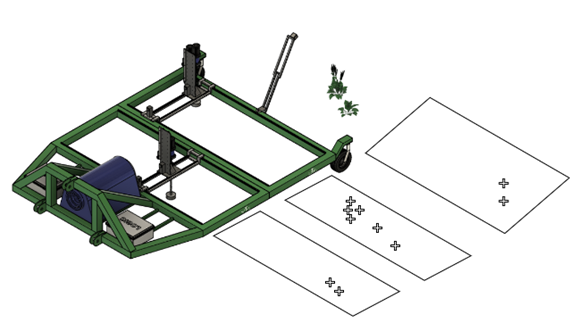
\includegraphics[width=0.7\linewidth]{gfx/ch03/nuga_cad.png}
    \caption{Nuga Platform}
    \label{fig:nuga-cad}
\end{figure}


% See classicthesis-config.tex for changing the prefixes of the refs
% Testing for autoref: \autoref{ch:intro}, \autoref{ch:examples}, and \autoref{sec:new}

%Testing for ``clever'' references: \cref{ch:intro} and \cref{ch:examples}
% Ugly work-around
% Part~\textsc{\ref{pt:showcase}}


\section{Simulation}\label{sec:simulation}
A representative simulation of reality is crucial for developing new algorithms and analyzing robot behavior before real-world implementation. Therefore, building a simulation of the project was a foundational step for this work, ensuring a controlled environment for validation and testing. Gazebo\footnote{Gazebo is a physics-based robotics simulation tool that allows testing and validation of robot models before real-world deployment. \url{https://gazebosim.org/home}} was the selected tool because it provides a physics engine, supports sensor and actuator modeling, and integrates well with ROS\footnote{ROS (Robot Operating System) is an open-source framework that provides tools, libraries, and conventions for developing, managing, and simulating robotic applications. \url{https://www.ros.org/}}, making it ideal for testing robotic systems.

The simulation consists of six key components: URDF files define the robot's structure and properties, SDF files describe the virtual environment, and Gazebo plugins provide additional functionality, such as simulating custom sensors, actuators, or control interfaces. Additionally, core system operations include joint control for managing the movement of the \ac{IT}, localization for tracking the robot’s position, and weed detection, which relies on an AI model for Rumex recognition. \autoref{fig:building-sim} illustrates these components as building blocks for the simulation.

\begin{figure}
    \centering
    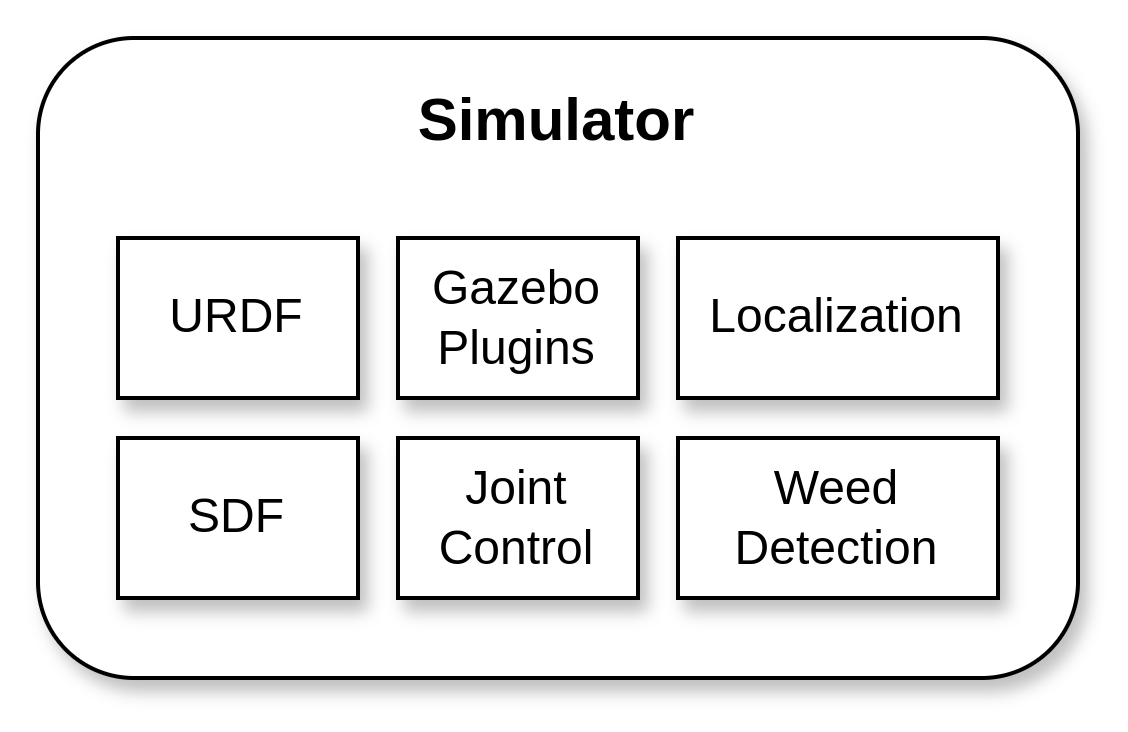
\includegraphics[width=0.5\linewidth]{gfx/ch03/simulator.png}
    \caption{Simulator Components}
    \label{fig:building-sim}
\end{figure}

\subsection{URDF}
\ac{URDF} is an XML file used to describe multibody systems for robot simulation. It defines the visual, collision, and inertial properties of rigid body objects, as well as their connections (\emph{joints}). This establishes a spatial relationship between frames, which ROS and Gazebo can later interpret for control and visualization. This file also allows modeling different types of sensors and incorporating Gazebo plugins to link it with ROS control actions. We exploit these capabilities to define camera intrinsics, IMU behavior, GPS properties, and control the \ac{IT} using \texttt{ros2\_control}\footnote{\texttt{ros2\_control} is a ROS 2 framework that provides a standardized interface for managing hardware, enabling modular and reusable control systems for robots. \url{https://control.ros.org/rolling/doc/getting_started/getting_started.html}}.

\autoref{fig:urdf-structure} displays the structure of the URDF files, being nuga the highest level entity that joins the robot description, gazebo sensor modeling and plugins, as well as \texttt{ros2\_control} configuration. Nuga description defines the robot's physical structure, including its links (e.g., chassis, wheels, camera support), joints (fixed, continuous, prismatic connections), sensors (cameras, IMU, GPS), and inertial properties. It organizes these components into a kinematic tree (e.g., base\_link -> chassis\_link -> wheels/sensors) using macros for modularity, and resulting in the model displayed in \autoref{fig:nuga-urdf}.

\begin{figure}[hbt]
    \myfloatalign
    \subfloat[URDF files structure.]
    {\label{fig:urdf-structure}
        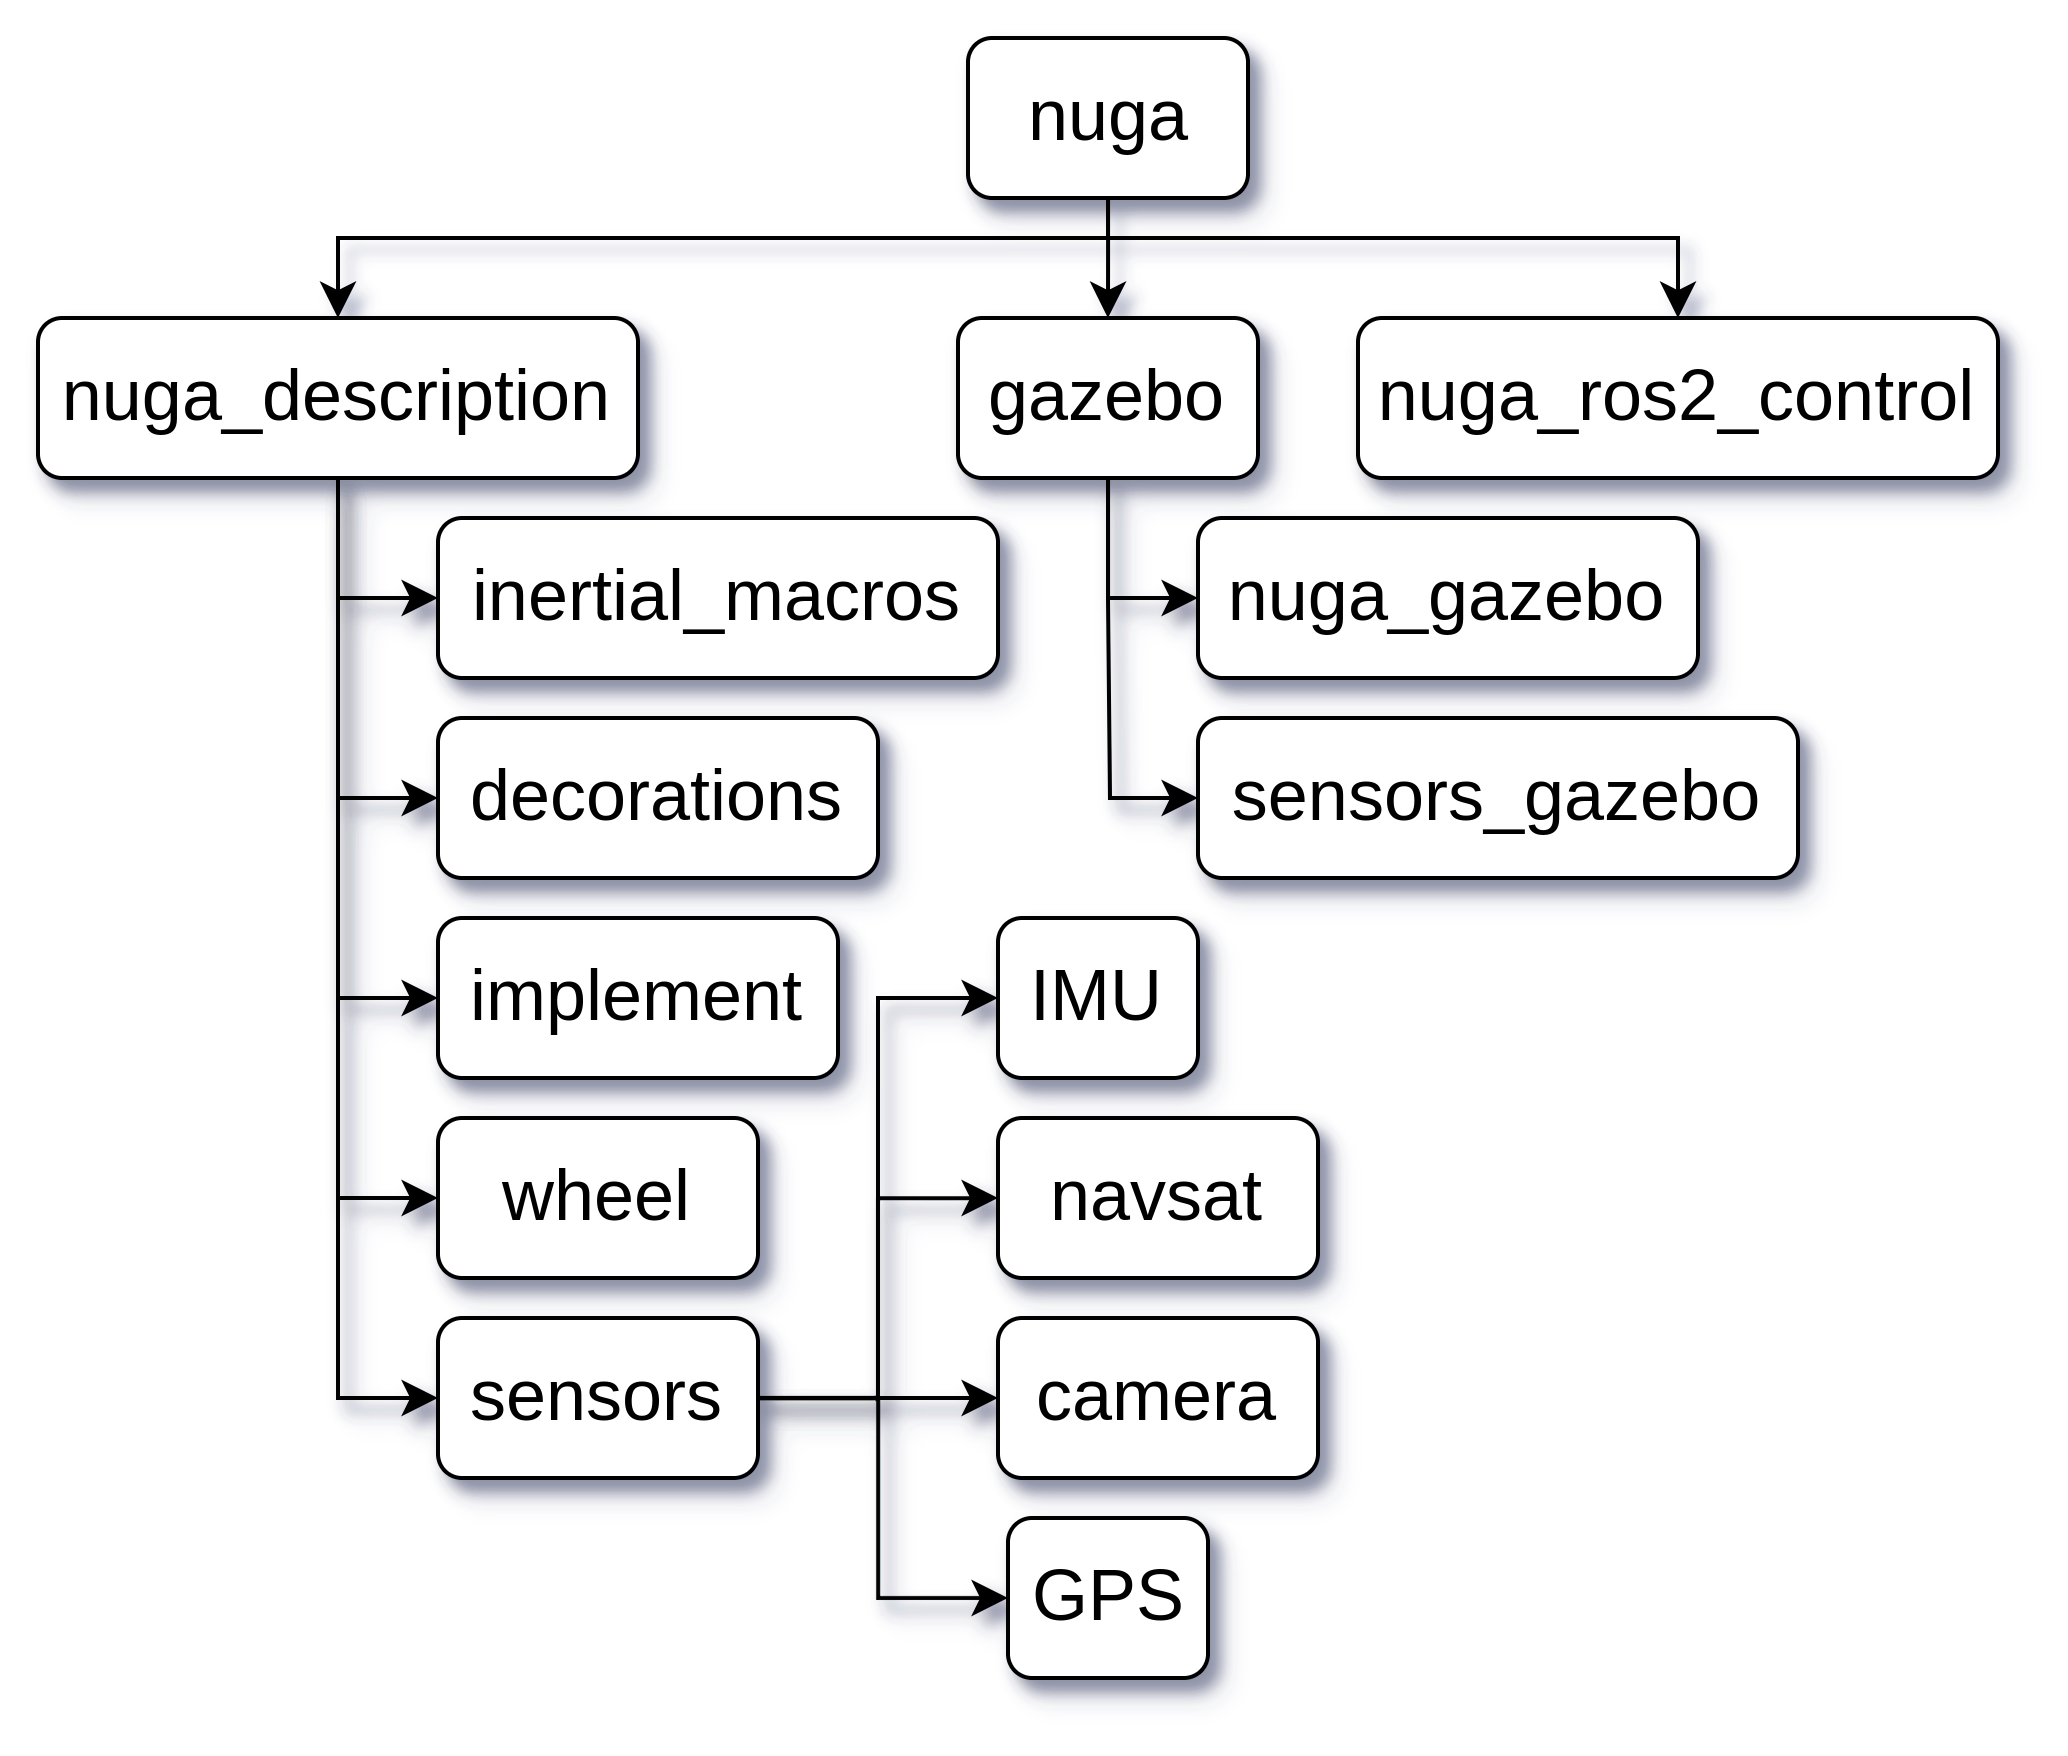
\includegraphics[width=.45\linewidth]{gfx/ch03/urdf.png}} \quad
    \subfloat[RViz visualization of Nuga description.]
    {\label{fig:nuga-urdf}%
        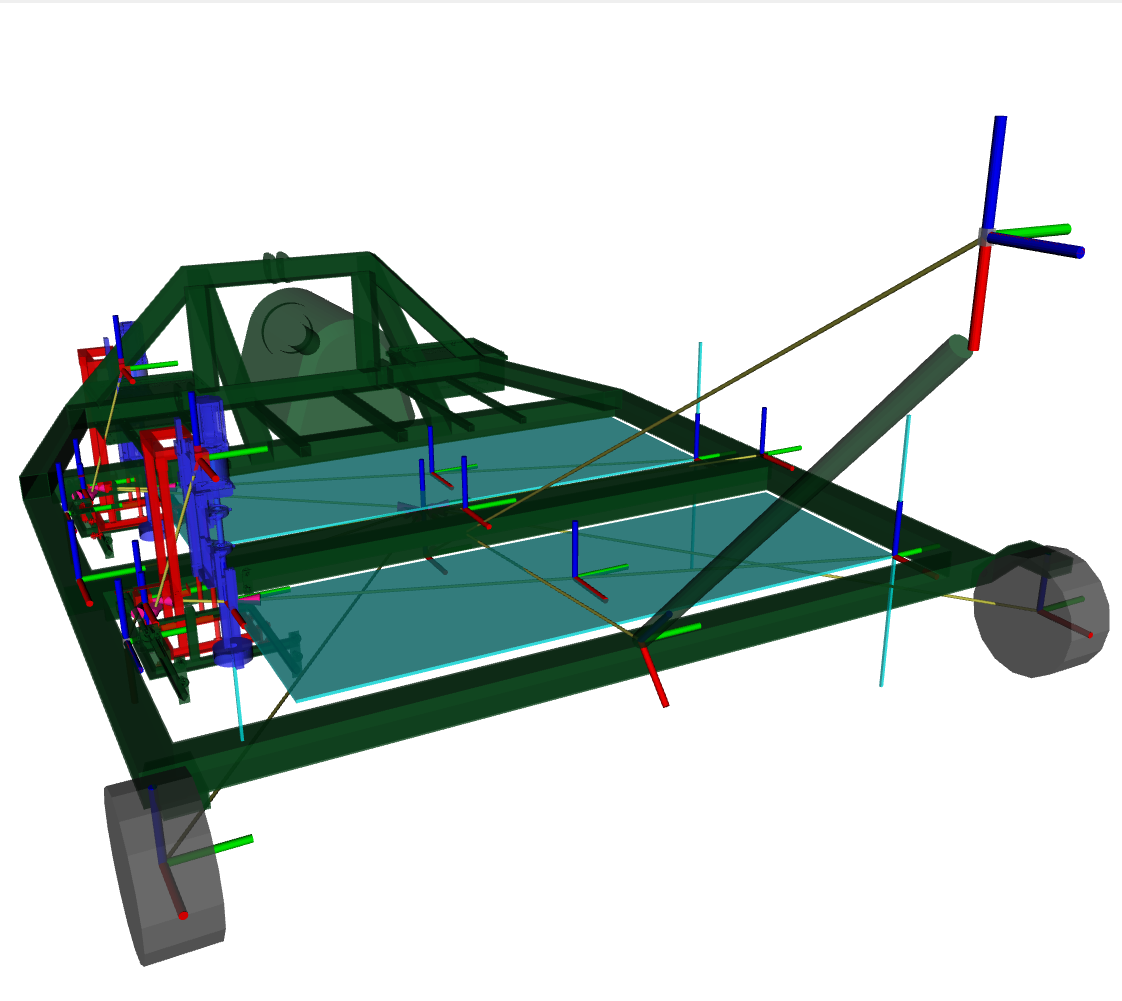
\includegraphics[width=.45\linewidth]{gfx/ch03/nuga_urdf.png}} \\
    \caption[Robot definition using URDF]{Robot definition using URDF}
\end{figure}

\subsection{SDF}
\ac{SDF} also written in XML, describes the properties of the virtual world. Gazebo uses this file to define the terrain, obstacles, lighting conditions, physics parameters, and other environmental elements that affect the robot’s interaction with the simulation. Having repeatability in a simulated world is important for debuging and testing purposes, for this reason a Python script was used to generate easy to configure worlds from a YAML configuration file. An example of the config file is shown in \autoref{lst:world-yaml}. For reproducibility, a seed value is configured in the simulation settings, the weed infestation pattern is defined within quadrants of specified dimensions (\texttt{quadrant\_size}) and each quadrant is individually configured with:

\begin{itemize}
    \item Spatial distribution:
          \begin{itemize}
              \item \textit{uniform}: Random uniform distribution
              \item \textit{clustered}: Random normal distribution with definable standard deviations ($\sigma_x, \sigma_y$)
          \end{itemize}
    \item Weed density: Weeds per square meter (weeds/m²)
    \item Direction: Propagation axis for adjacent quadrants ($\pm x,\pm y$)
    \item Workspace expansion: If \texttt{outside\_workspace} is true, the infestation area extends 10\% beyond the quadrant boundaries.
\end{itemize}

A visual result of the generated world using such configuration file is shown in \autoref{fig:world}.

\begin{figure}[h]
    \centering
    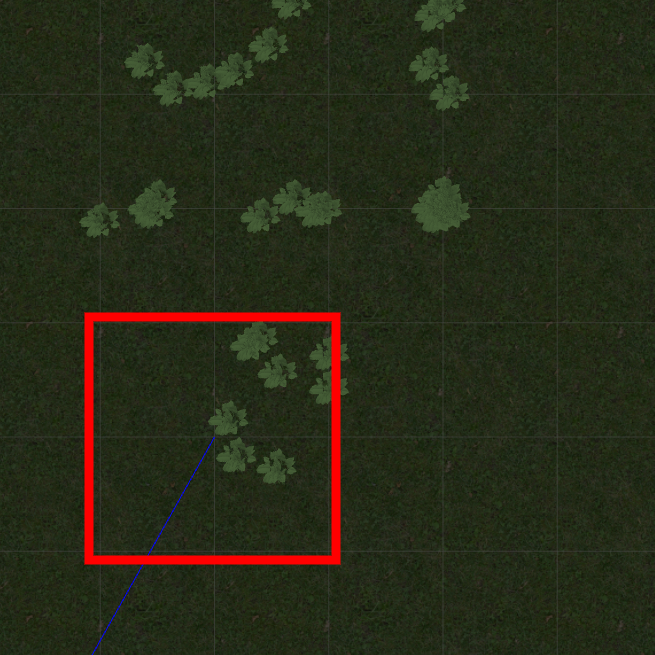
\includegraphics[width=0.4\linewidth]{gfx/ch03/world.png}
    \caption{Weed Infestation Example}
    \label{fig:world}
\end{figure}

\subsection{Gazebo Plugins}
The files \texttt{nuga\_gazebo} and \texttt{sensors\_gazebo} from \autoref{fig:urdf-structure} instantiate and configure Gazebo plugins to define sensor behavior, including optical properties for the camera, as well as update rates and noise models for the IMU and GPS. The file \texttt{nuga\_ros2\_control} on the other hand, establishes an interface between the \ac{IT} 's joints and \texttt{ros2\_control} framework, specifying the command interface (position), controller type (forward position controller), and movement limits, enabling 3-\ac{DOF} prismatic motion for each tool. Regarding movement control of the Nuga vehicle, the \texttt{ros\_planar\_move} plugin satisfied all control requirements given the platform's kinematic constraints, eliminating the need for additional configuration.

\subsection{Joint Control}
The control of both \ac{IT} units was handled using the \texttt{ros2\_control} framework (configuration example shown in \autoref{lst:ros2_control-yaml}), as previously described. This framework provides a seamless transition between simulation and real hardware control. In this context, the \texttt{forward\_command\_controller} was used, which is recommended for simulation because it bypasses PID computations by directly sending commands to simulated joints. These joints already track positions perfectly, without the disturbances or error correction needed in real-world scenarios. Simulators like Gazebo inherently handle ideal position tracking, making closed-loop control redundant. However, when switching to real hardware, replacing it with a \texttt{position\_controller} is needed but straightforward thanks to the flexibility of the framework.

Nuga's workspace layout and dimensions are shown in \autoref{fig:ws}. The gantry carrying the \ac{IT} operates within a zone of $2.09$ m in the $Y$ direction, $0.72$ m in $X$, and $0.26$ m in $Z$. An extraction cycle begins with the gantry moving in $X$ and $Y$ to position the tool above the plant, followed by a downward movement in $Z$ to lower the drill and perform the extraction. The gantry has a maximum speed of $1\frac{m}{s}$ in the $XY$ plane, and each extraction can take up to $45$ seconds per plant.

\begin{figure}[t]
    \myfloatalign
    \subfloat[$X,Y$ Workspace]
    {\label{fig:xy-ws}
        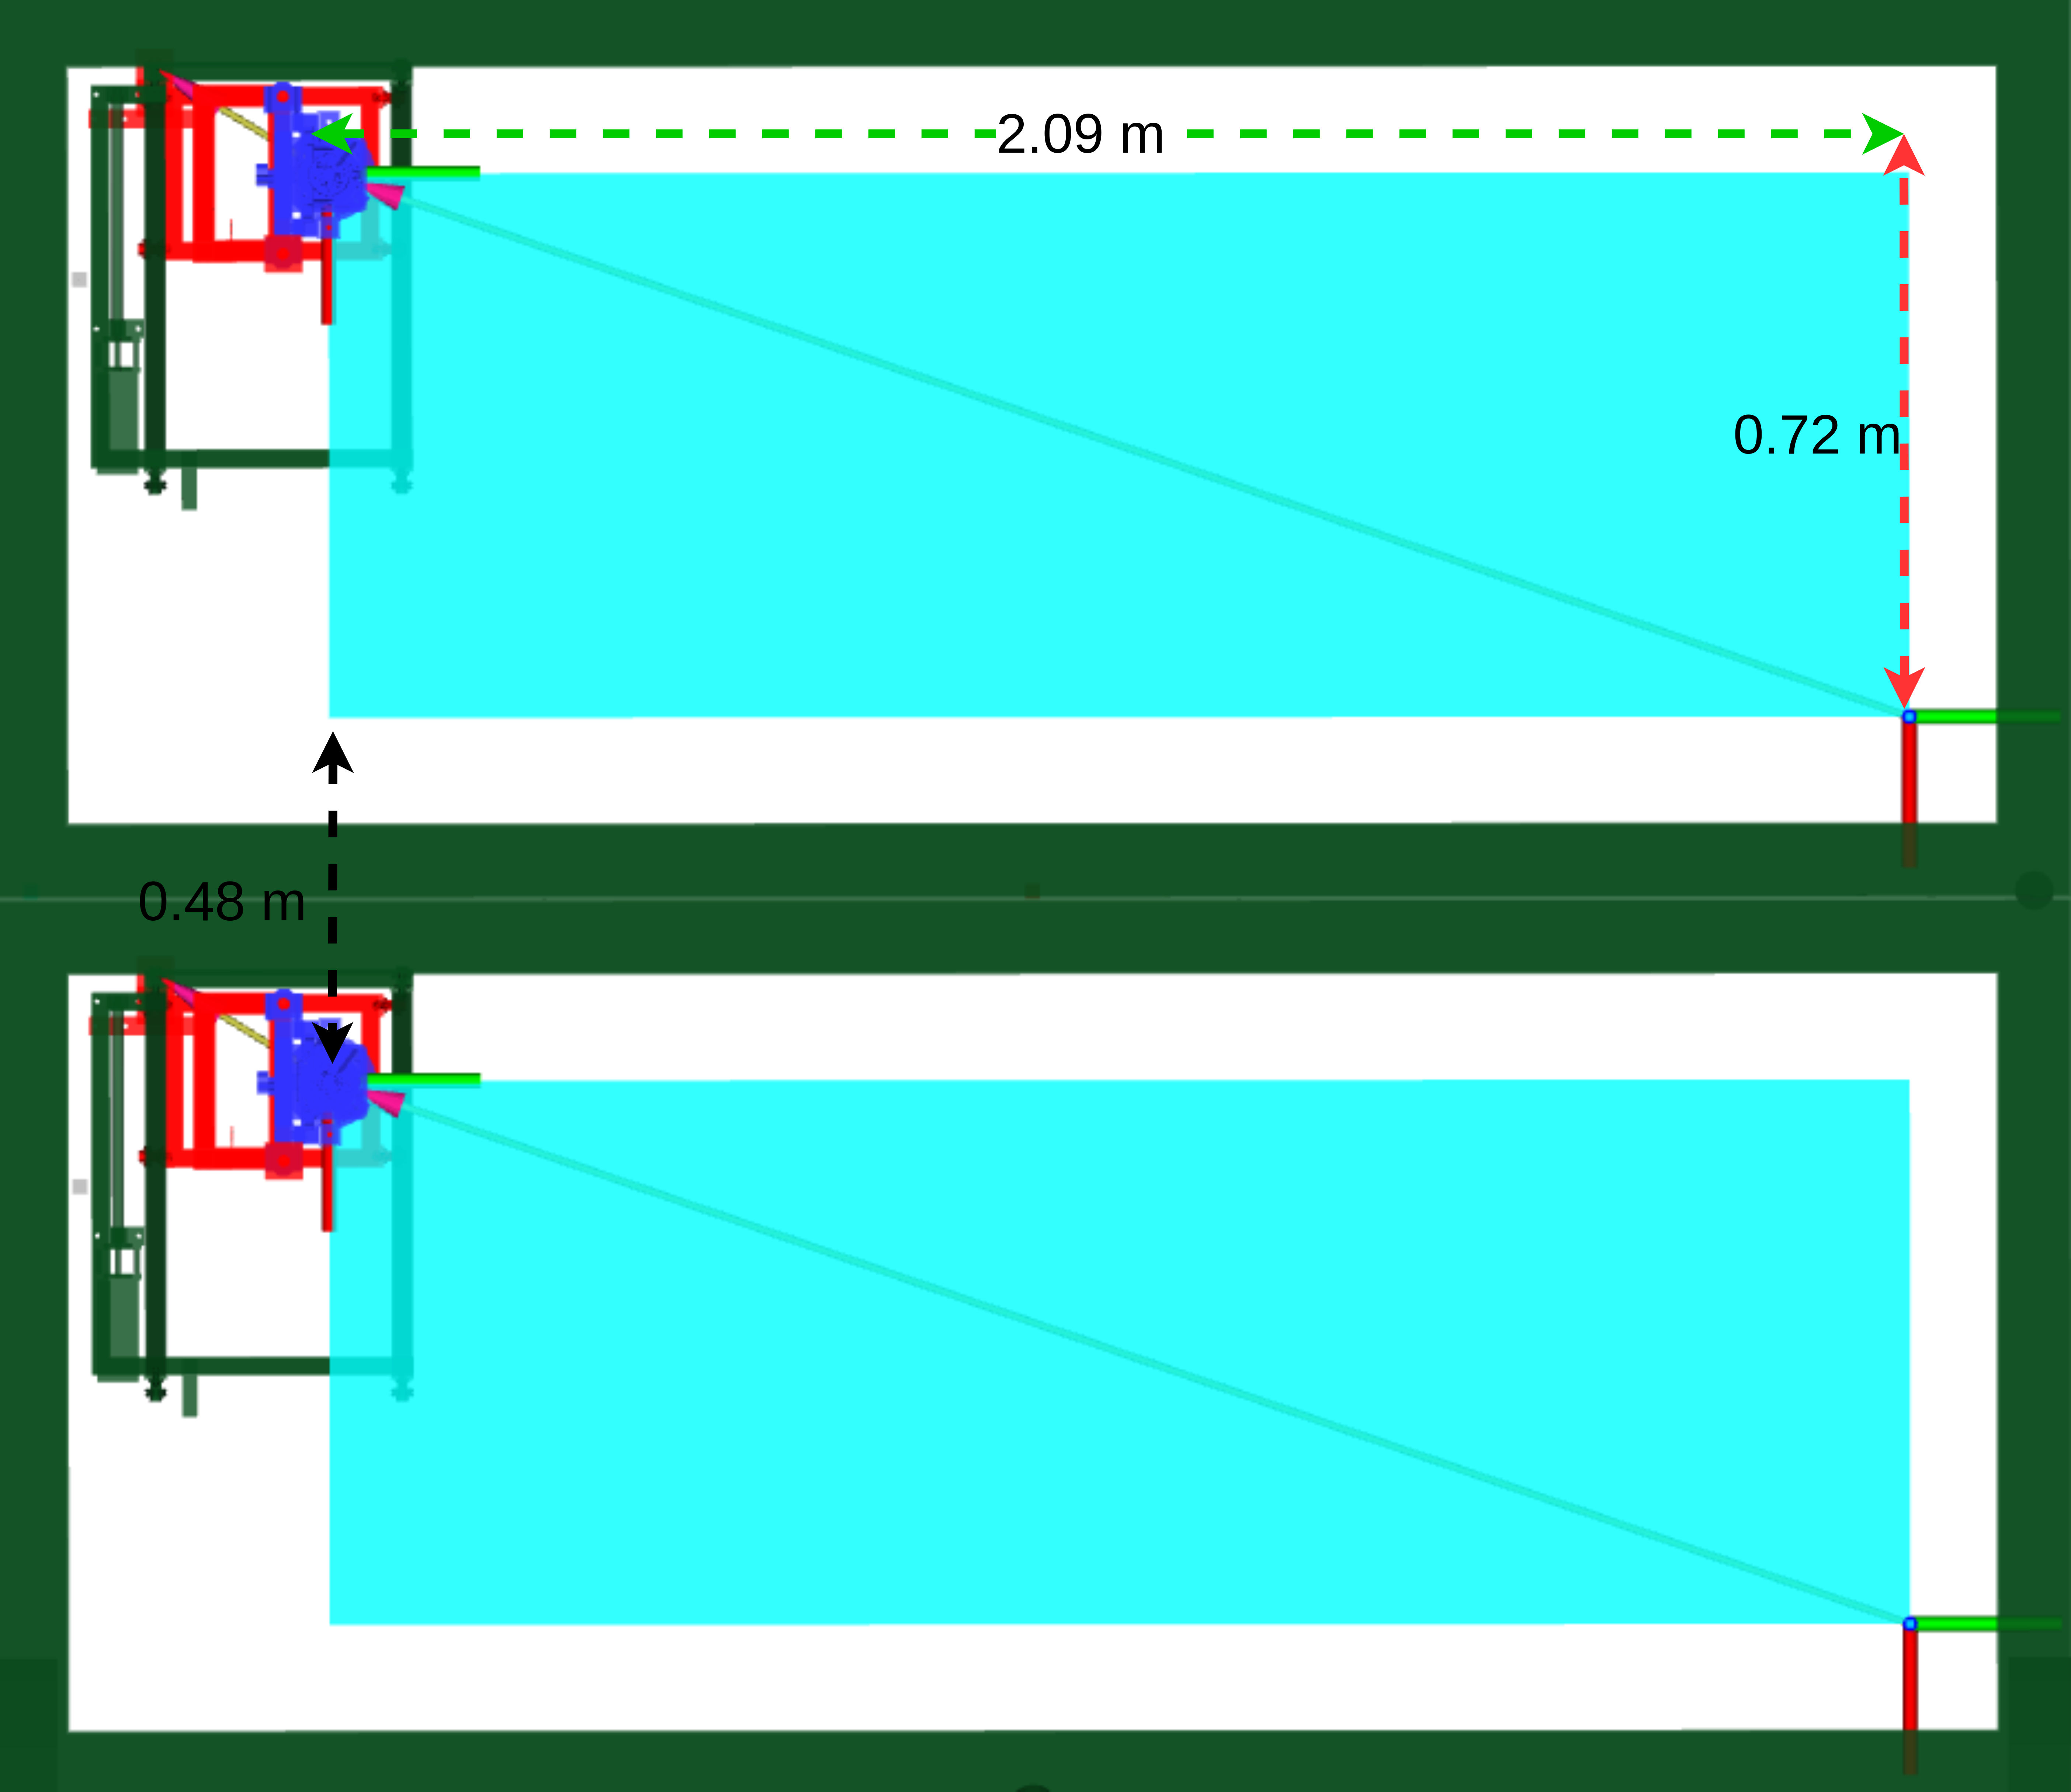
\includegraphics[width=.45\linewidth]{gfx/ch03/xy_ws.png}} \quad
    \subfloat[$Z$ Workspace]
    {\label{fig:z-ws}%
        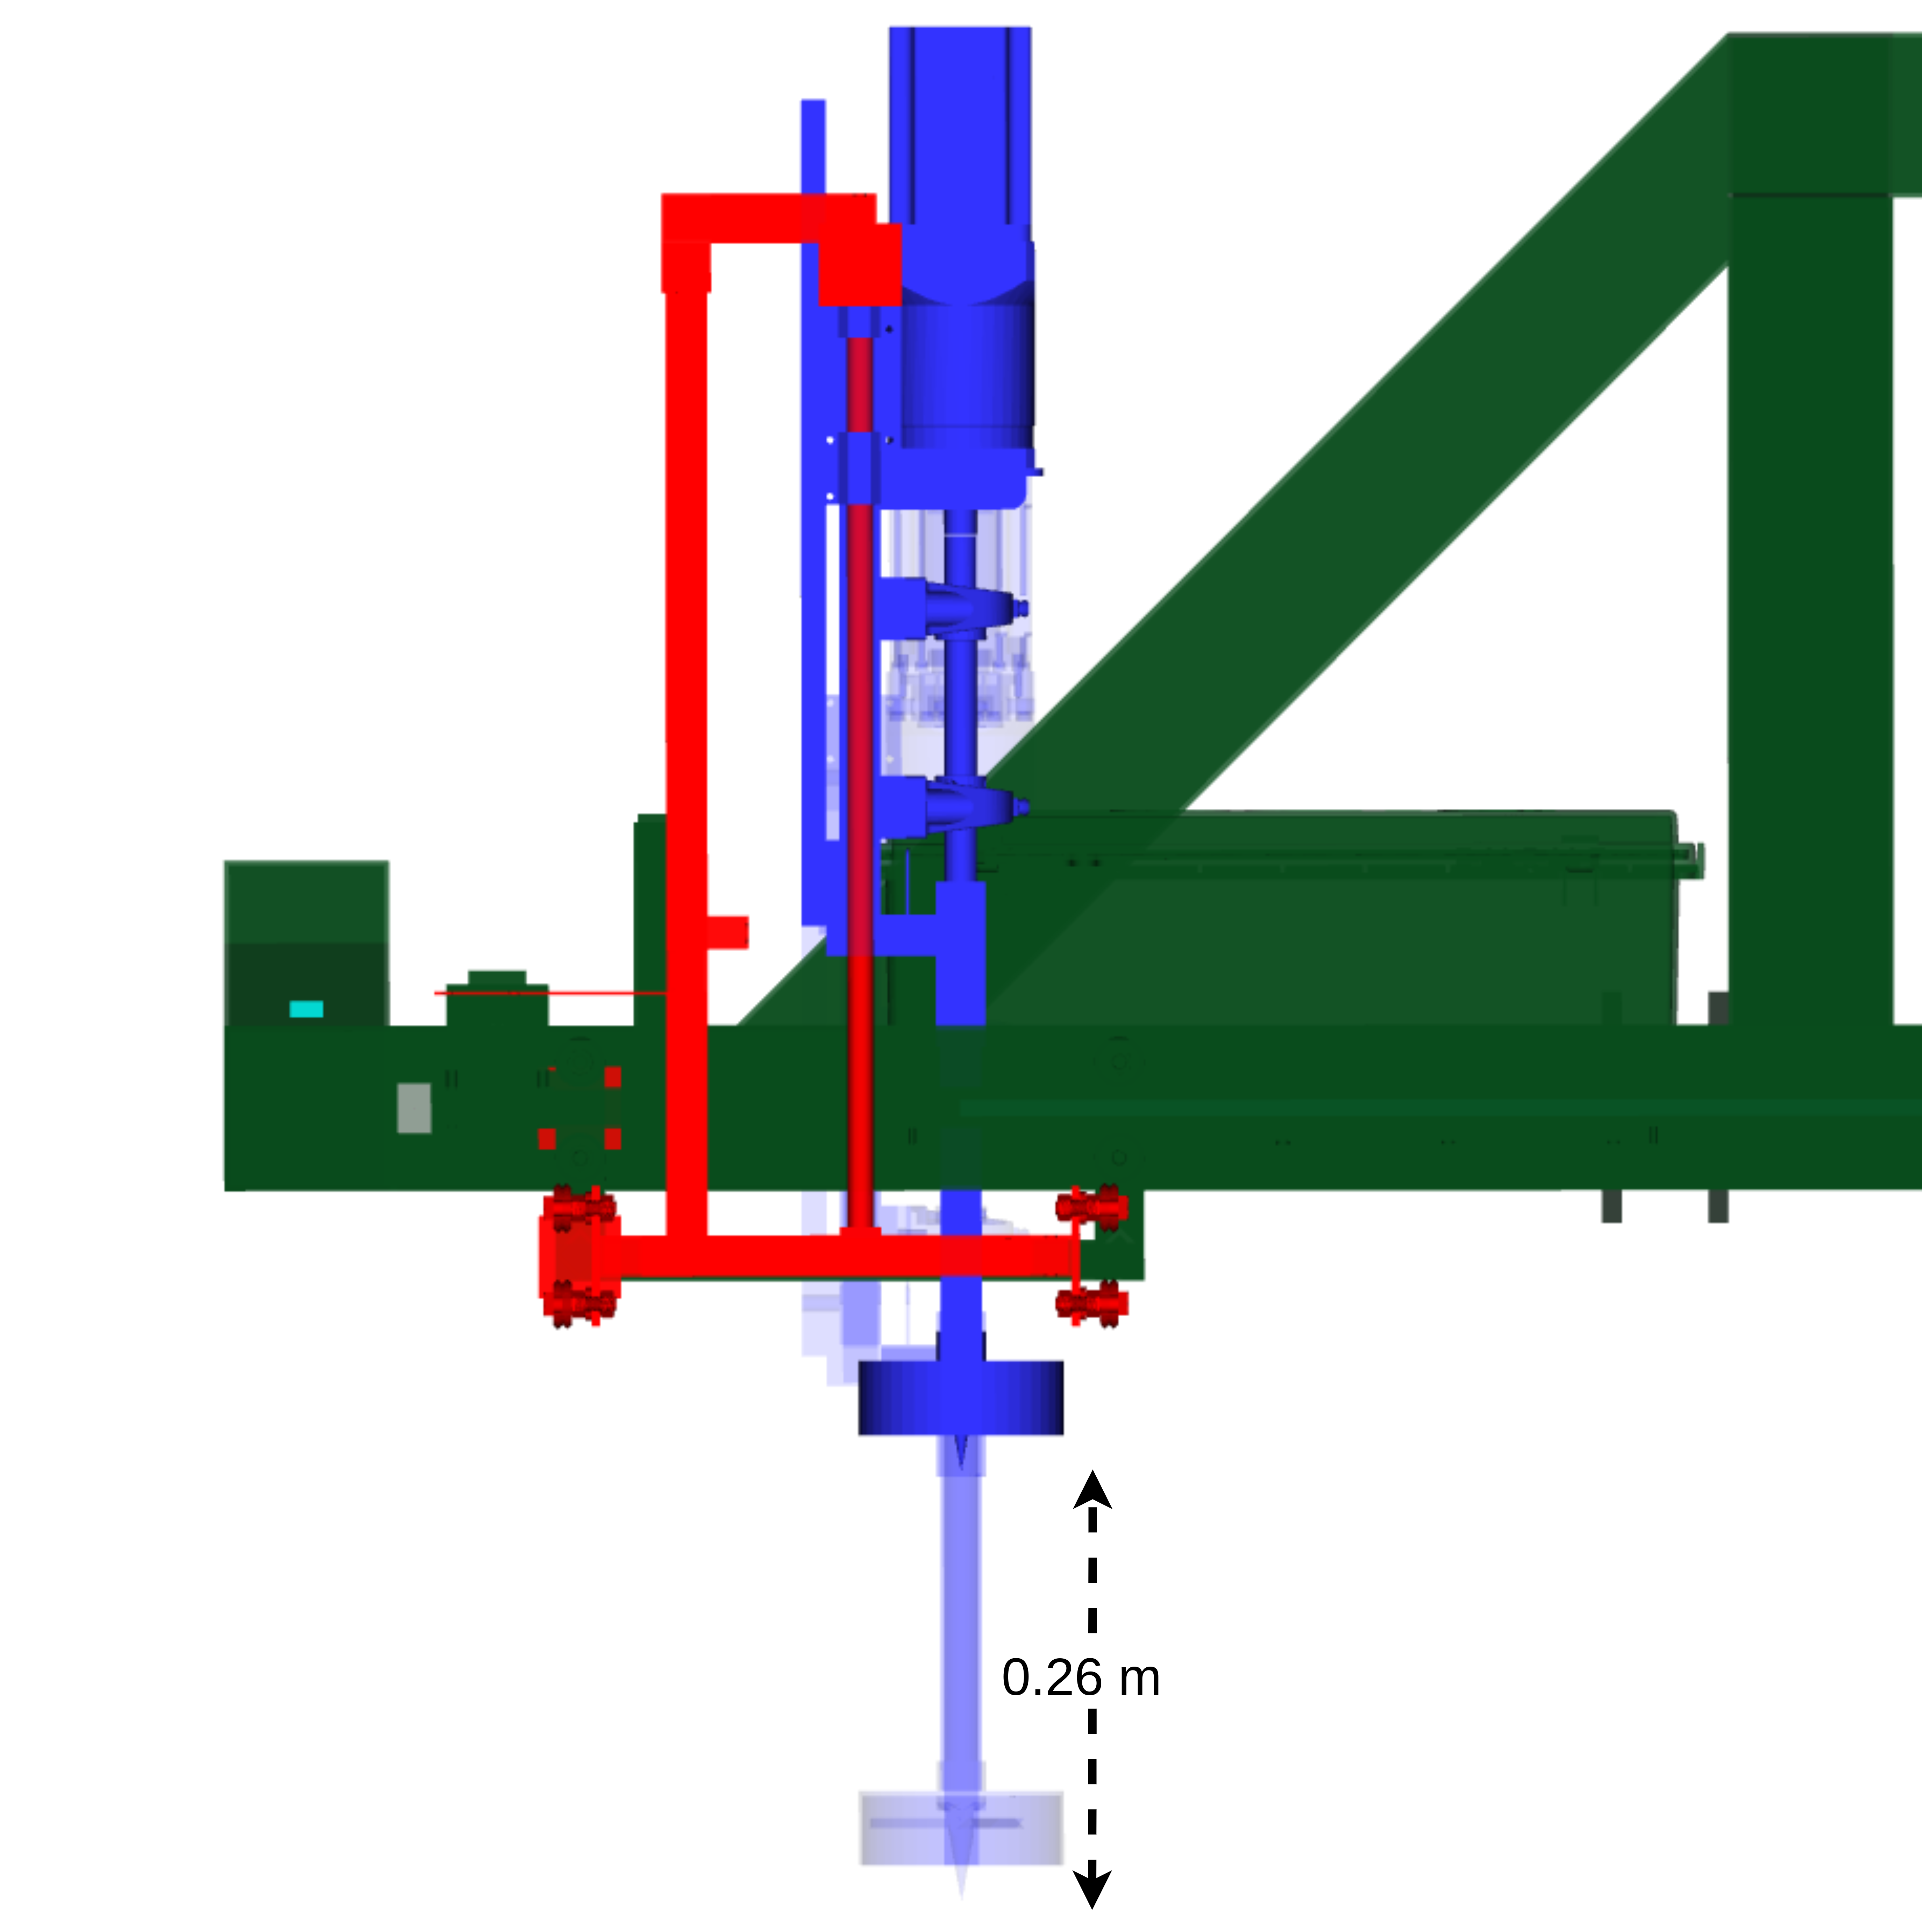
\includegraphics[width=.45\linewidth]{gfx/ch03/z_ws.png}} \\
    \caption{\ac{IT} Workspace Layout}\label{fig:ws}
\end{figure}

The \ac{IT} is controlled using ROS$2$ actions, which provide a structured way to handle asynchronous tasks with feedback and result reporting. For the $XY$ movement of the gantry, the \texttt{AxisPosition} action is used, allowing the specification of target coordinates ($x$, $y$) and speed, while providing feedback on the current position and confirming whether the target was reached. The \texttt{Extraction} action manages the vertical movement of the tool along the $Z$ axis, reporting the depth reached, total time taken, and success status, along with real-time feedback on the current depth. Finally, the \texttt{ExtractionCycle} action coordinates the execution of multiple extractions by accepting an array of target poses and their corresponding IDs, providing feedback on the current status and reporting the results of the extraction process for each pose. These actions enable precise and modular control of the gantry system, ensuring efficient and reliable operation. A diagram summarizing this process is shown in \autoref{fig:gantry-control}.

\begin{figure}[h]
    \centering
    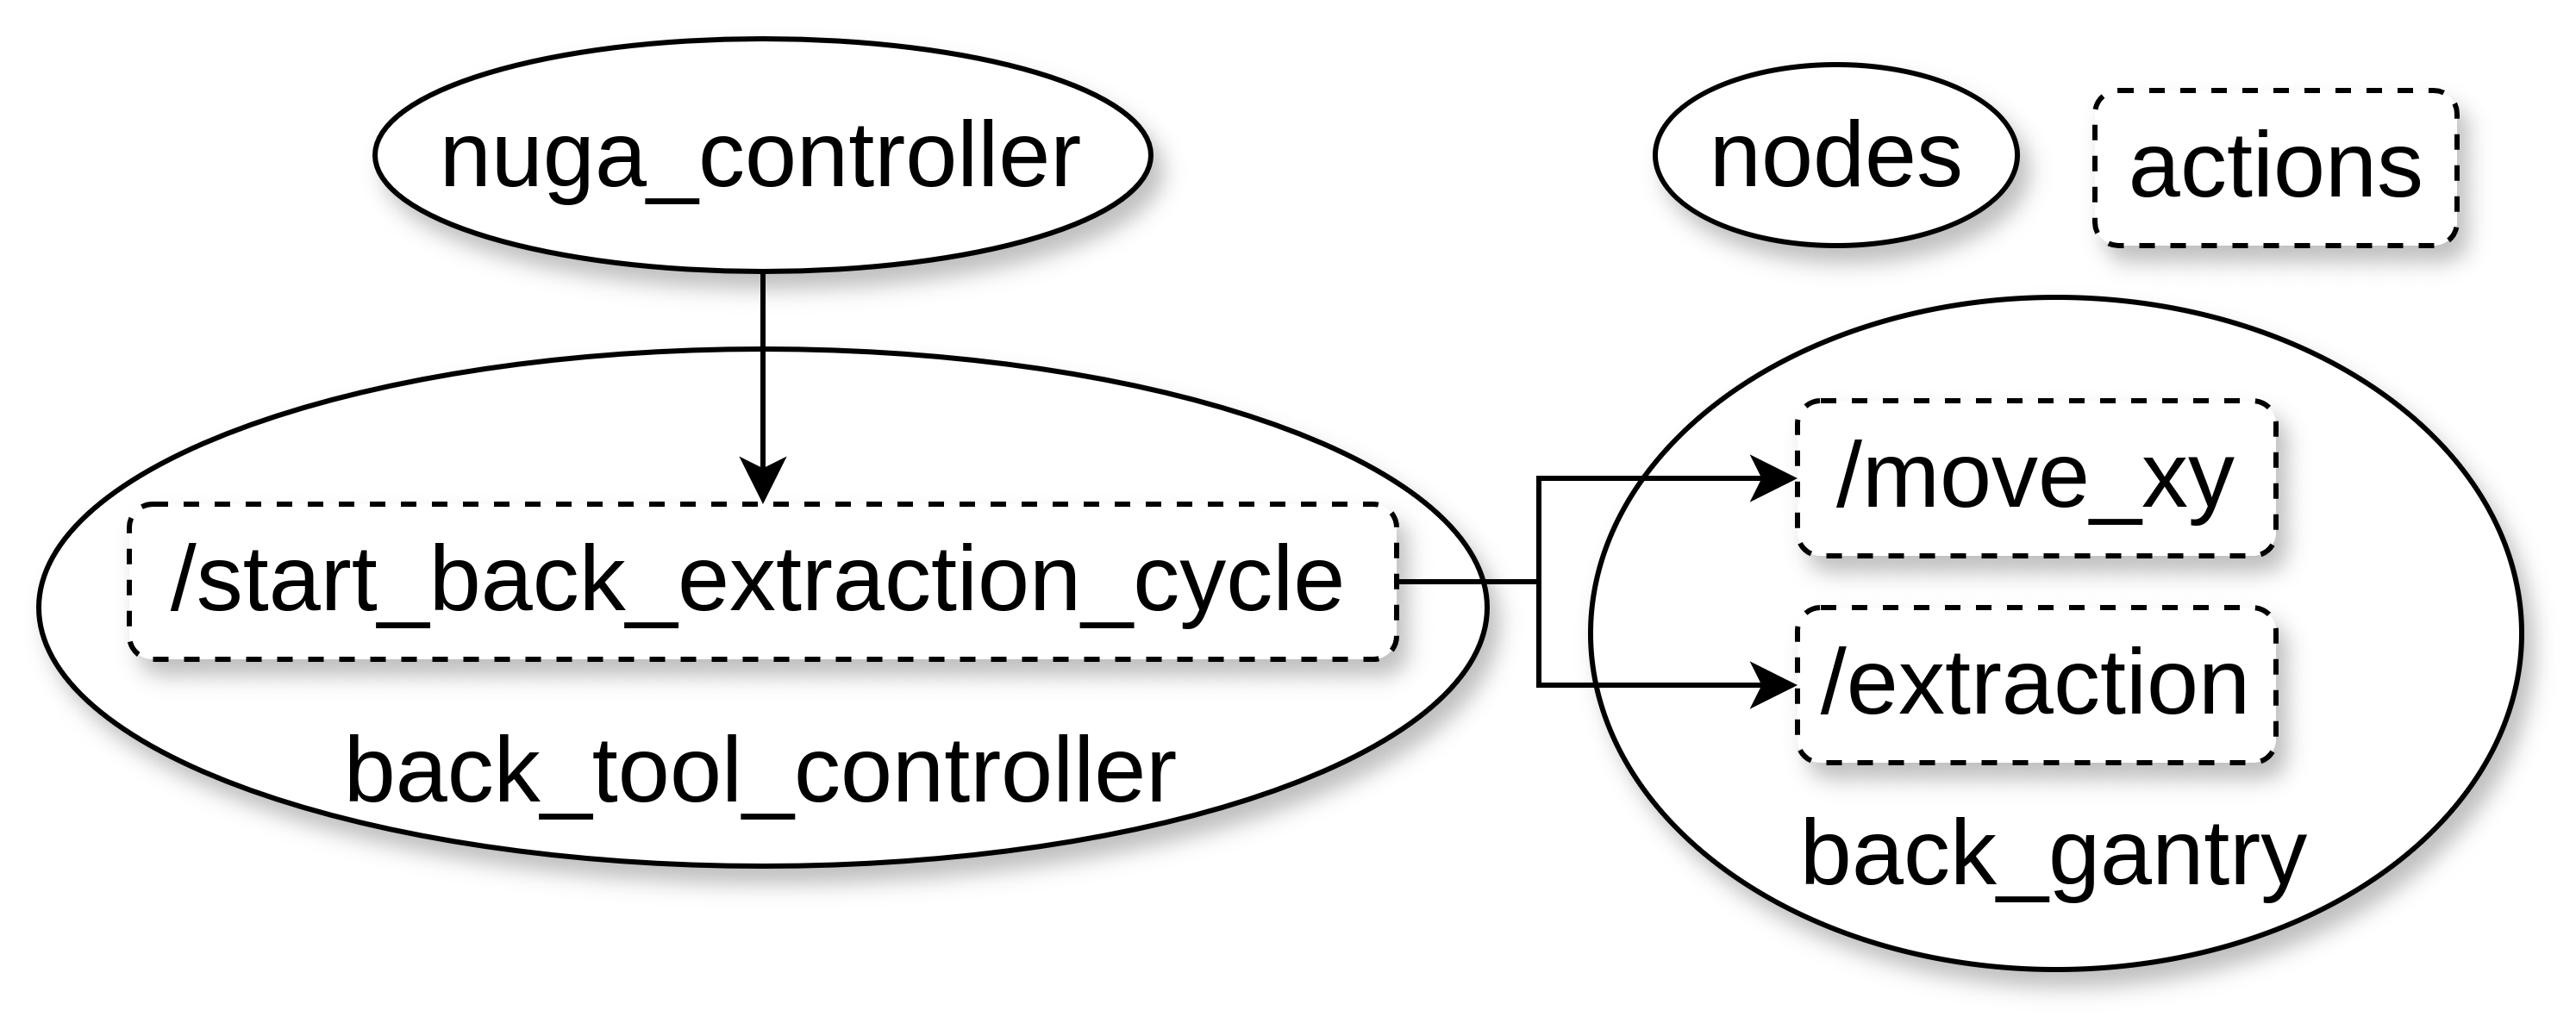
\includegraphics[width=0.7\linewidth]{gfx/ch03/gantry_control.png}
    \caption{ROS Interface for back gantry control}
    \label{fig:gantry-control}
\end{figure}


\subsection{Localization}
Accurate localization is essential for mobile robot navigation. In most robotic systems, a combination of sensors such as wheel encoders, IMU's, and GPS (for outdoor applications) are used to estimate the robot's pose in the environment. In simulation, these sensors can be approximated to real-world conditions and provide a testbed for validating higher-level behaviours (e.g., path planning, task allocation, etc.). In this work, the \texttt{robot\_localization}\footnote{\texttt{robot\_localization} is a collection of state estimation nodes, each of which is an implementation of a nonlinear state estimator for robots moving in 3D space. It contains two state estimation nodes, \texttt{ekf\_localization\_node} and \texttt{ukf\_localization\_node}. In addition, it provides \texttt{navsat\_transform\_node}, which aids in the integration of GPS data. \url{https://docs.ros.org/en/melodic/api/robot_localization/html/index.html}} package was used to estimate the robot's pose by fusing sensor data. Typically, this would involve:

\begin{itemize}
    \item An \textbf{Extended Kalman Filter (EKF)} fusing high-frequency wheel odometry and IMU data with low-frequency GPS.
    \item A \texttt{navsat\_transform\_node} to convert GPS data into the robot's odom frame.
\end{itemize}

However, as wheel odometry was not implemented in the simulation due to plugin limitations, the navigation was done merely using fusion of GPS and IMU, this allowed the EKF to still function and produce a pose estimate. While this approach deviates from standar practice, it was deemed acceptable for this thesis for several reasons: Localization is not the primary contribution of this work, the fused GPS and IMU data provided sufficient accuracy and stability for validating the \ac{TA} investigation, and the use of \texttt{robot\_localization} still maintains a realistic pipeline for future extension of real-world deployment.

This setup does not model short-term drift correction that would normally be provided by wheel odometry, and the reliance on GPS alone may introduce small jumps or inaccuracies in pose estimation. These limitations are acknowledged but do not affect the core objectives or validity of the experiments conducted in this work.

\subsection{Weed Detection}
Paltech uses an in-house machine learning model for Rumex recognition, trained on a dataset of images captured under various lighting conditions. The model is integrated into the simulation using a ROS2 node that subscribes to the camera topic and publishes detection results. This node processes camera images, applies the trained model, and outputs the detected plants’ positions in camera coordinates along with confidence scores. This integration enables real-time detection of Rumex within the simulated environment, supporting planning and execution of extraction tasks. The model’s training dataset includes images such as the one shown in \autoref{fig:rumex-trainning}, and it is capable of generalizing to simulation images, as illustrated in \autoref{fig:rumex-sim}.

\begin{figure}[htb]
    \myfloatalign
    \subfloat[Trainning dataset image]
    {\label{fig:rumex-trainning}%
        \includegraphics[width=.45\linewidth]{gfx/ch03/rumex.png}} \quad
    \subfloat[Weed detection in simulation]
    {\label{fig:rumex-sim}
        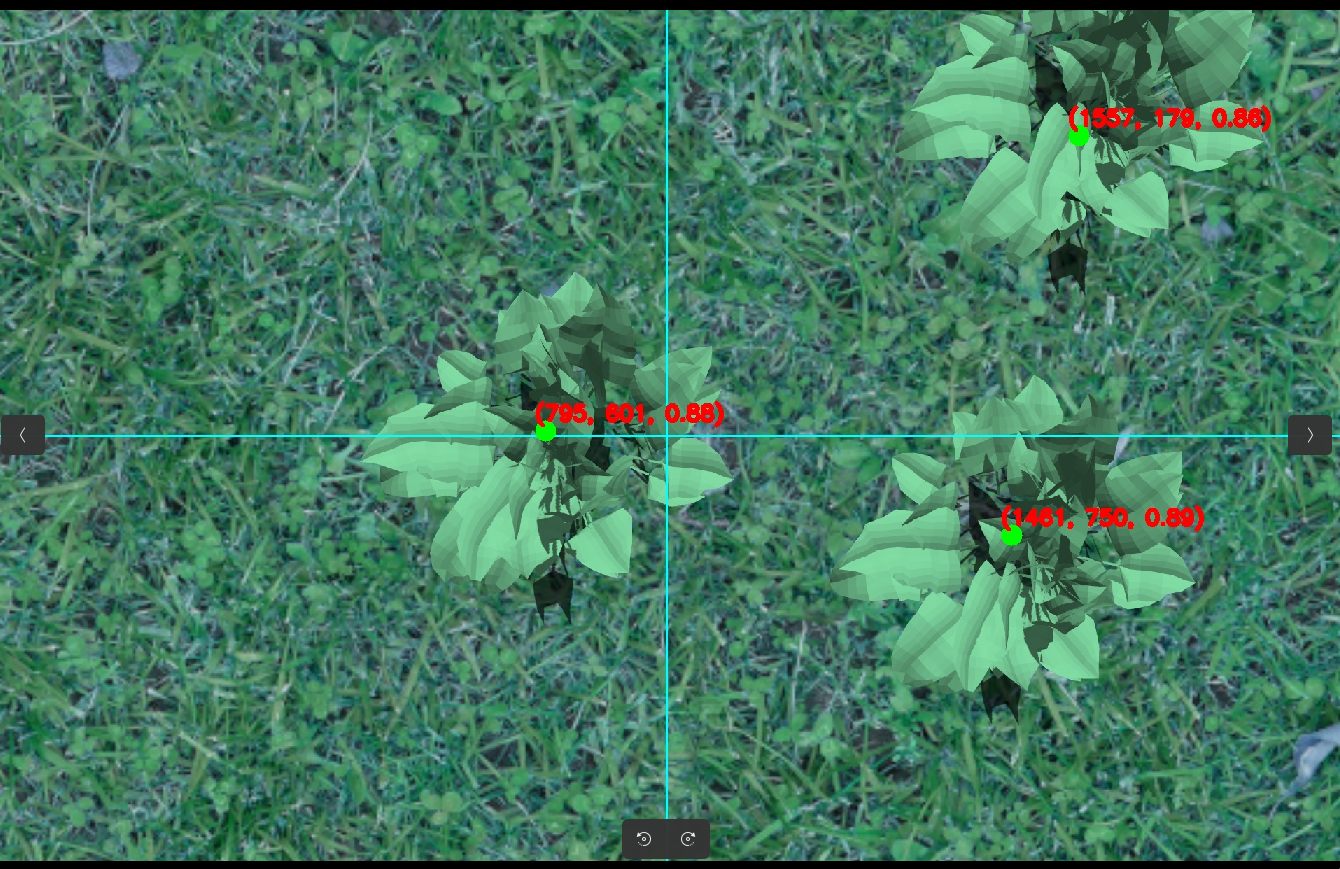
\includegraphics[width=.45\linewidth]{gfx/ch03/rumex_sim.png}} \\
    \caption{Example of trainning and detection}\label{fig:rumex-example}
\end{figure}

\subsection{Nuga Controller}
The Nuga controller is the main node responsible for orchestrating the movement of the robot, managing the \ac{IT} units, and performing task allocation based on the weed positions received from the detection node. A high-level overview of the controller's operation is shown in \autoref{fig:nuga-controller}. The timer callbacks \texttt{get\_ws\_limits()} and \texttt{get\_imp\_offsets()} are self-destructive timers used to retrieve the positions of the tool workspace limits and their offsets relative to the \texttt{base\_link}. Once this information is received, the timers are destroyed. The same applies to the callback of the \textit{/head\_camera/camera\_info} topic, which is used to obtain the camera’s central pixel position for later use.

\begin{figure}[ht]
    \centering
    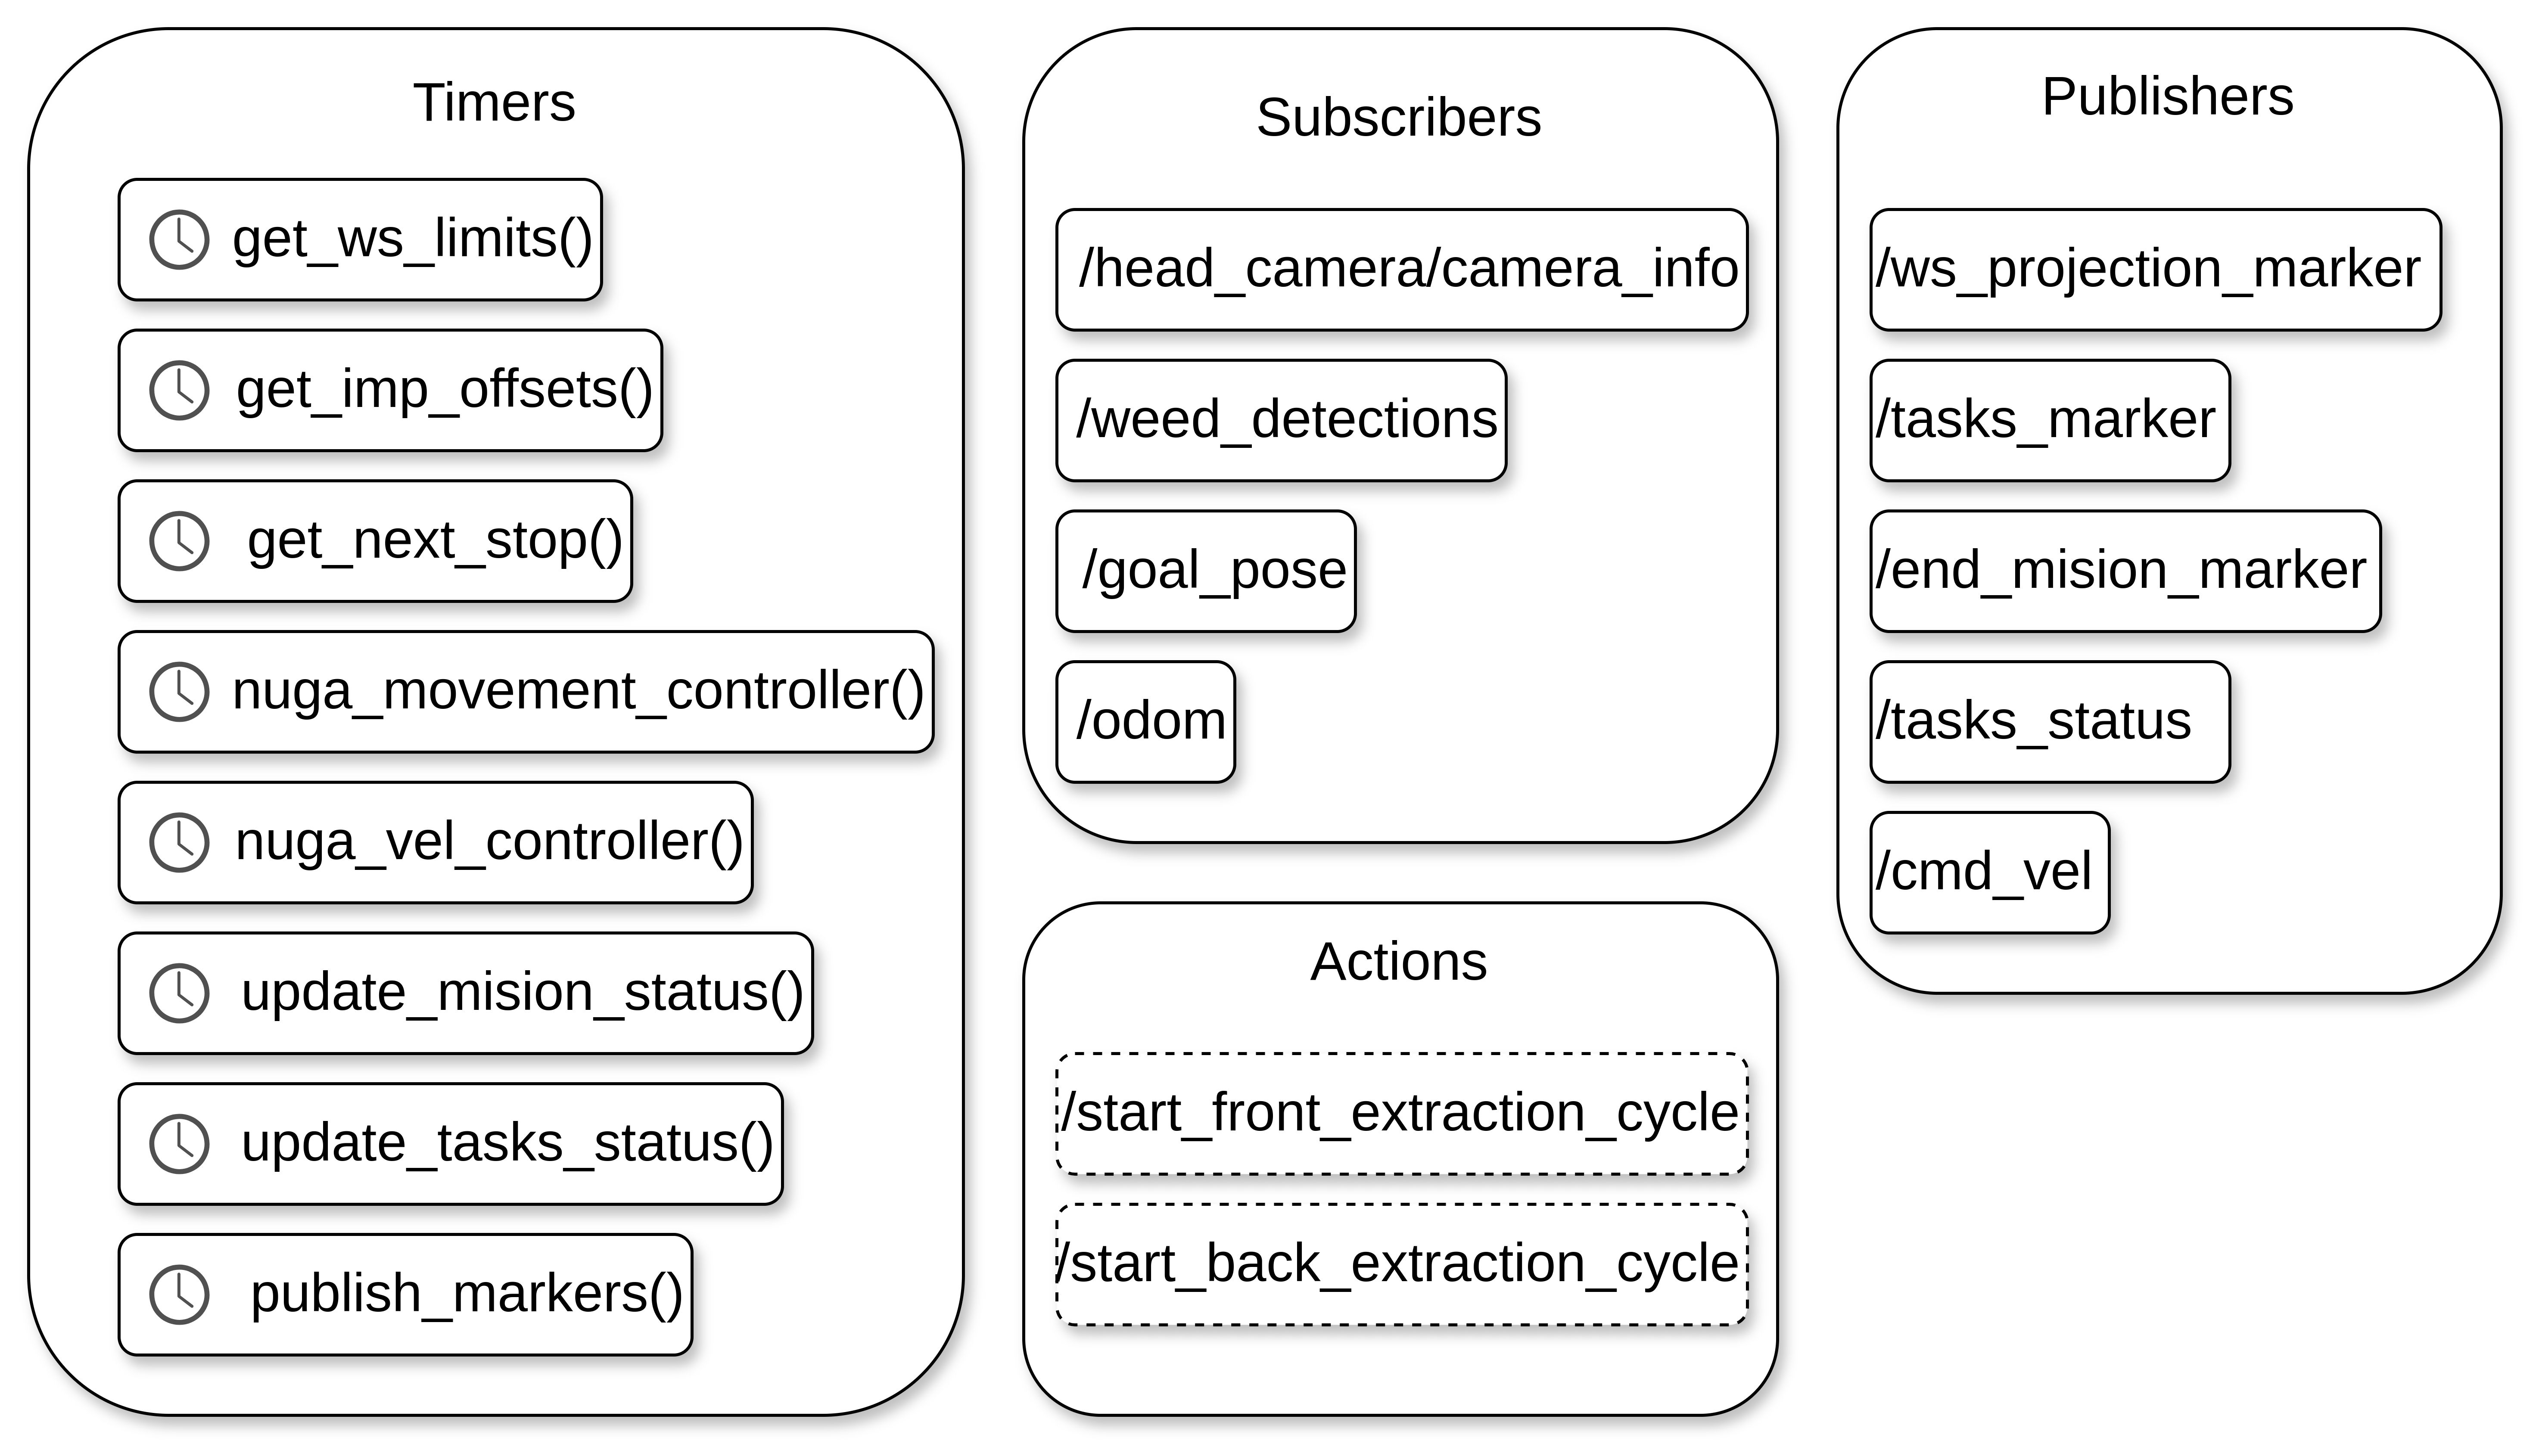
\includegraphics[width=0.95\linewidth]{gfx/ch03/nuga_controller.png}
    \caption{Nuga Controller ROS Interface}
    \label{fig:nuga-controller}
\end{figure}

The \texttt{get\_next\_stop()} function is a timer callback that computes the robot's next stop when required. It uses the current detections, the robot's pose, and the selected task allocation algorithm to determine the next target position, as well as the tasks to be executed at that stop by each \ac{IT}. The execution steps followed by this method are shown in Algorithm \ref{alg:get-next-stop}.

Once a stop is determined, Nuga’s movement and velocity controllers govern the robot’s behavior. The \texttt{nuga\_movement\_controller()} function switches the robot’s state between \textit{stationary} and \textit{moving} when needed, while also measuring the time spent in each state. If the robot reaches the target position, this method stops the robot and triggers the actions required to perform the extraction cycle; otherwise, it keeps the robot in the \textit{moving} state. Finally, \texttt{nuga\_velocity\_controller()} takes the robot’s state and computes the necessary velocity commands, publishing them to the \textit{/cmd\_vel} topic.

The callback \texttt{update\_mission\_status()} continuously checks whether the robot has reached the end-of-mission position in order to stop it and generate log information for mission metrics. On the other hand, \texttt{update\_tasks\_status()} continuously publishes the status of all weed detections to the \textit{/tasks\_status} topic. These tasks can include those assigned to the back or front tool, current detections, tasks outside the future path, and failed tasks.

Finally, \texttt{publish\_markers()} updates RViz markers to visualize robot position and task status. \autoref{fig:rviz-visualization} shows an example of the RViz visualization in a usual mission.

\begin{figure}[H]
    \centering
    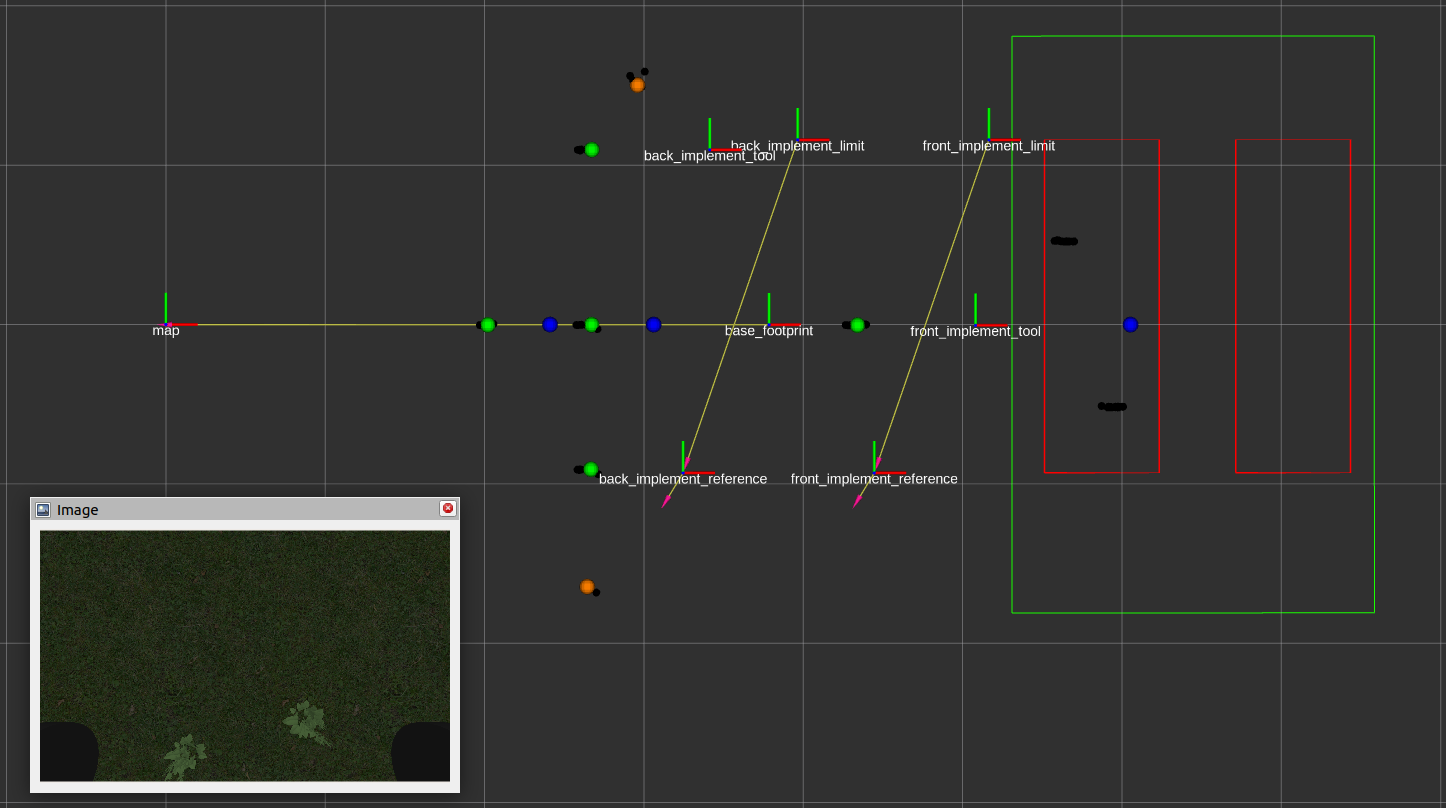
\includegraphics[width=0.95\linewidth]{gfx/ch03/rviz_black_1.png}
    \caption{RViz Visualization}
    \label{fig:rviz-visualization}
\end{figure}

\paragraph{\autoref{fig:rviz-visualization}} Displays the current position of the robot (\texttt{base\_link}), the tool workspaces, and tool positions using coordinate frames. Task categories are indicated with colored spheres: green for successful tasks, orange for tasks outside the path, red for failed tasks, and blue for robot stops. The workspace projections of the onboard tools are shown using red rectangles, while the green rectangle represents the front camera’s field of view.

\section{Task Allocation}
Paltech currently offers its weeding solutions in fields ranging from $0.5$ to $20$ hectares, with an average weed density of $0.4$ to $2.0$ weeds/m$^2$. \autoref{fig:field-weed-density} shows an example of usual weed density in a 1-hectare field, while \autoref{fig:field-path-planning} illustrates the coverage path planning pattern that the robot follows in the same field. The simulations in this thesis are limited to the linear movements shown in \ref{fig:field-path-planning}, due to the motion constraints described at the beginning of \autoref{sec:TA}. As a result, the simulation environments were designed accordingly.

\begin{figure}[H]
    \myfloatalign
    \subfloat[Weed density]
    {\label{fig:field-weed-density}
        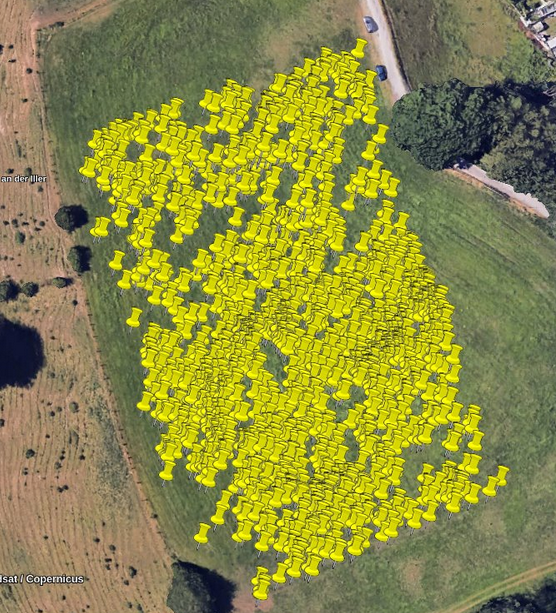
\includegraphics[width=.41\linewidth]{gfx/ch03/field_weed_density.png}} \quad
    \subfloat[Coverage path planning pattern]
    {\label{fig:field-path-planning}%
        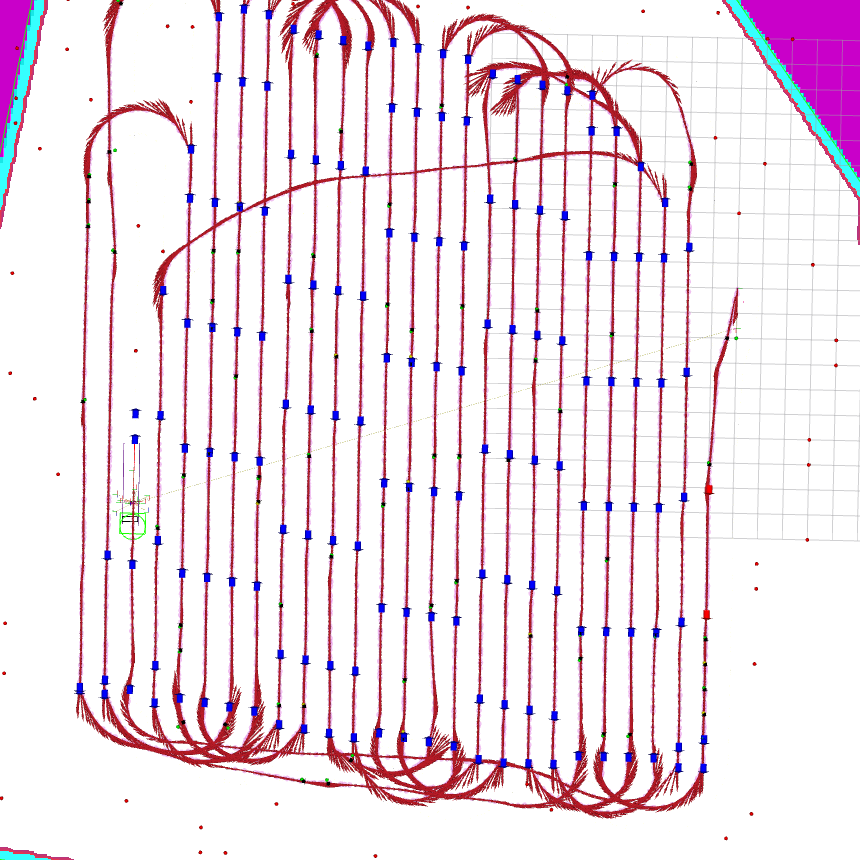
\includegraphics[width=.45\linewidth]{gfx/ch03/field_path_planning.png}} \\
    \caption{Weed distribution and coverage path in an agricultural field}\label{fig:usual-field-example}
\end{figure}

\subsection{Simulation Setup}
Simulations were customized using YAML files, as mentioned in \autoref{sec:simulation}, allowing for ease of configuration and logging convenience. All tests took place in a rectangular grass field of $10\text{m} \times 50\text{m}$, with different weed densities along a straight strip of $2\text{m} \times 50\text{m}$, simulating one line of the coverage path planning (observe an example in \autoref{fig:sim-example}). The local weed distribution within each quadrant ($2\text{m} \times 2\text{m}$) varied in both type (\textit{uniform} or \textit{clustered}) and density, replicating irregular Rumex growth.

\begin{figure}[hbt]
    \centering
    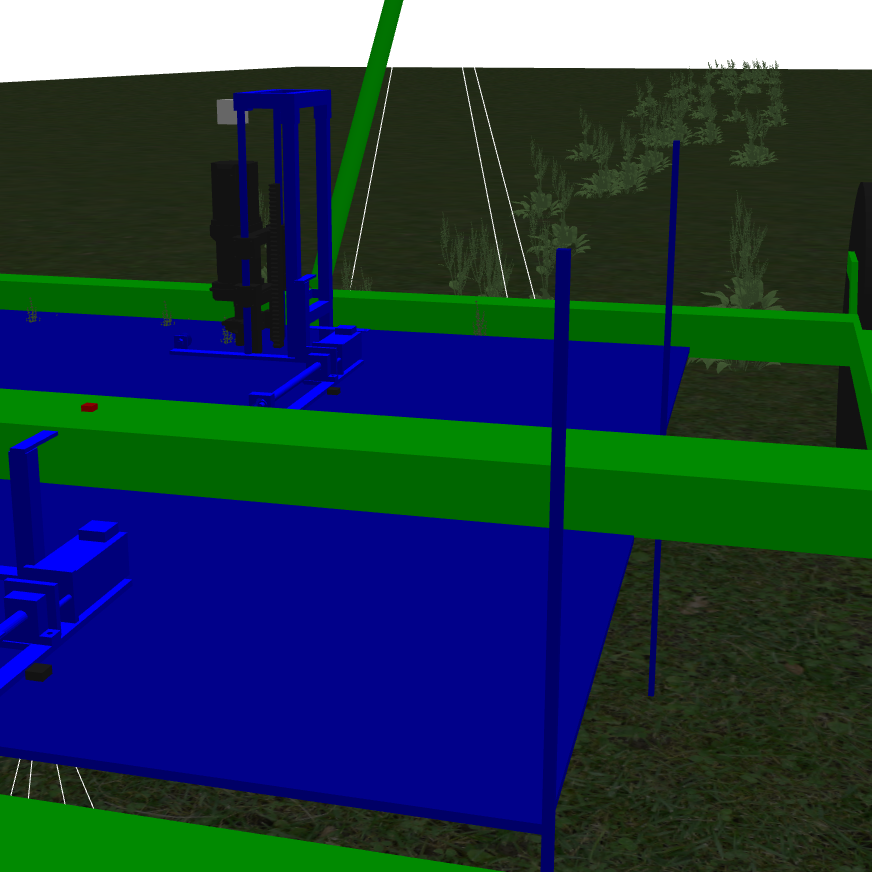
\includegraphics[width=0.5\linewidth]{gfx/ch03/field_strip_path_2.png}
    \caption{Simulation Example}
    \label{fig:sim-example}
\end{figure}

\subsection{Algorithm Comparison}
The first simulation corresponds to an infestation area of $100\text{m}^2$, with a weed density of $0.28$ weeds/m$^2$. This simulates a low weed density scenario, as shown in \autoref{fig:task-visualization-low-density}. \autoref{fig:results-low-density} presents both the task visualization and the mission metrics comparison across algorithms.

The first two missions in \autoref{fig:mission-metrics-low-density} represent the baseline method using one and two tools, respectively. This comparison was made only to determine the natural improvement in mission time when adding an additional tool, even with a non-optimized algorithm. Missions three, four, and five correspond to the graph search, optimization, and market-based approaches, respectively. We observe similar mission times and no significant improvement over the baseline method, which is expected since the weed density is low and, most of the time, the separation between weeds prevents the robot from reaching them with both tools simultaneously. Nevertheless, we observe a reduction in tool idle time with algorithms three, four, and five. The heuristic algorithm results in an idle time of $12.8$ min. for the front tool, whereas the others remain within the range of $8$ min. to $9.8$ min.

\begin{figure}[htb]
    \myfloatalign
    \subfloat[Task Visualization]
    {\label{fig:task-visualization-low-density}
        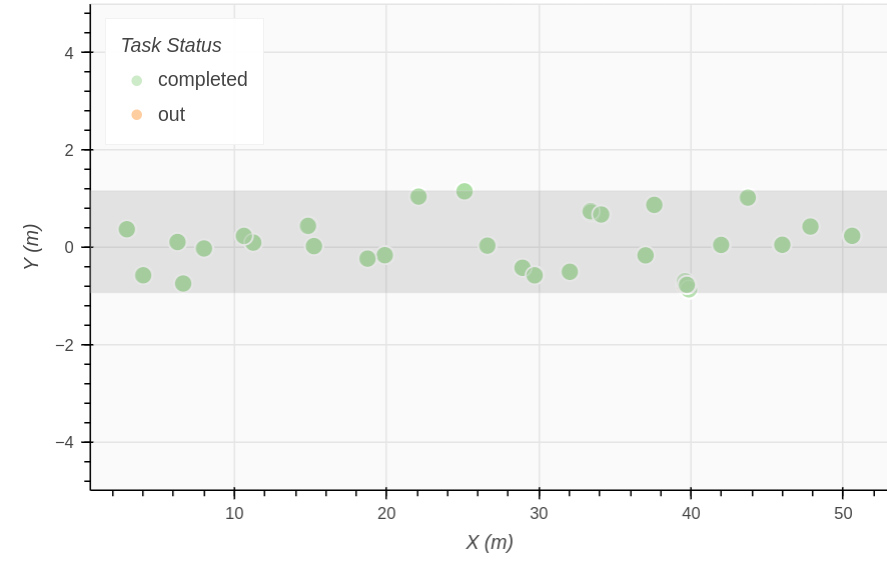
\includegraphics[width=.45\linewidth]{gfx/ch03/50m_low_density_tasks.png}} \quad
    \subfloat[Mission Metrics]
    {\label{fig:mission-metrics-low-density}
        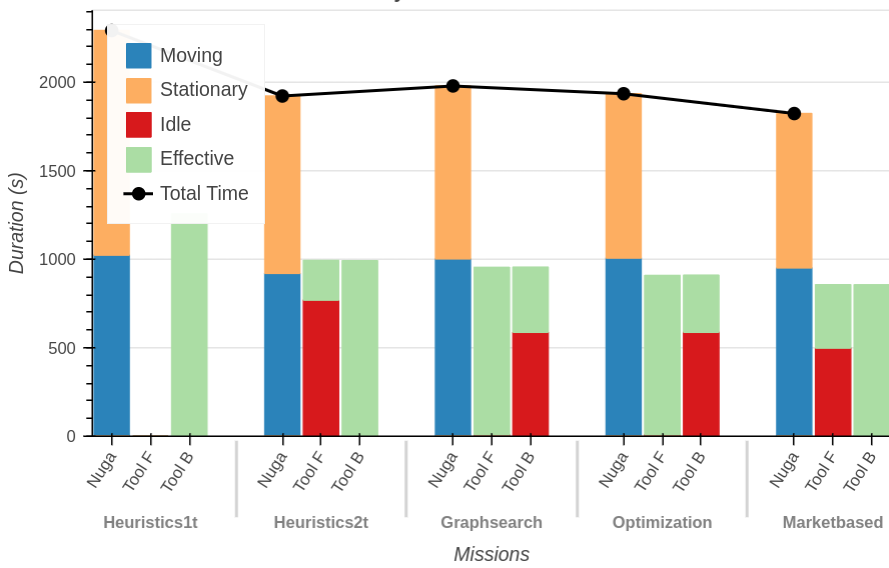
\includegraphics[width=.45\linewidth]{gfx/ch03/50m_low_density_missions.png}} \\
    \caption{Low density algorithms comparison}\label{fig:results-low-density}
\end{figure}

For the second simulation, we increased the average weed density to $0.55$ weeds/m$^2$, simulating a medium-density scenario, as shown in \autoref{fig:task-visualization-medium-density}. In \autoref{fig:mission-metrics-medium-density}, we observe improvements in both mission time and tool productivity. Both the graph search and optimization-based algorithms show improvements compared to the heuristic approach. Specifically, while the baseline method overuses the back tool, resulting in high idle time for the front tool, graph search and optimization achieve more balanced tool usage. The market-based algorithm also reduces idle time, although not as significantly as the other two methods.

\begin{figure}[htb]
    \myfloatalign
    \subfloat[Task Visualization]
    {\label{fig:task-visualization-medium-density}
        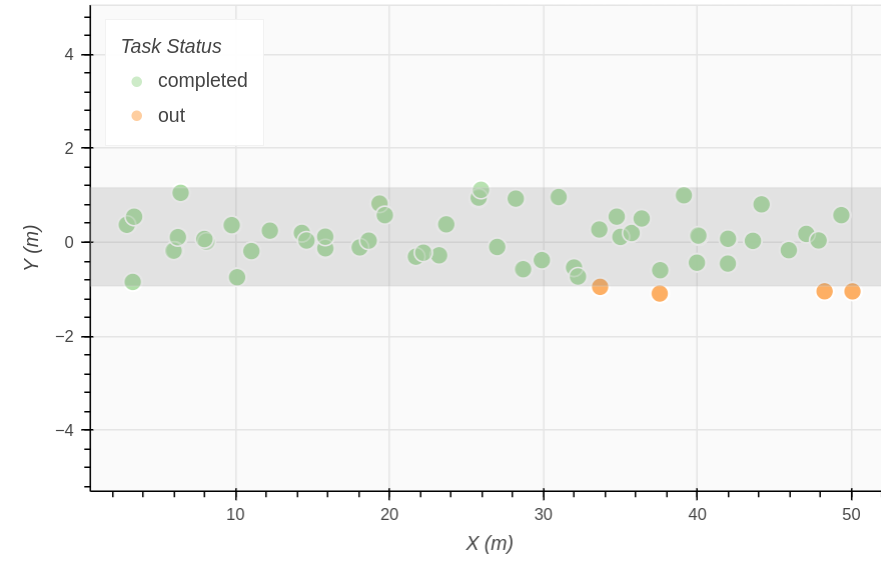
\includegraphics[width=.45\linewidth]{gfx/ch03/50m_medium_density_tasks.png}} \quad
    \subfloat[Mission Metrics]
    {\label{fig:mission-metrics-medium-density}
        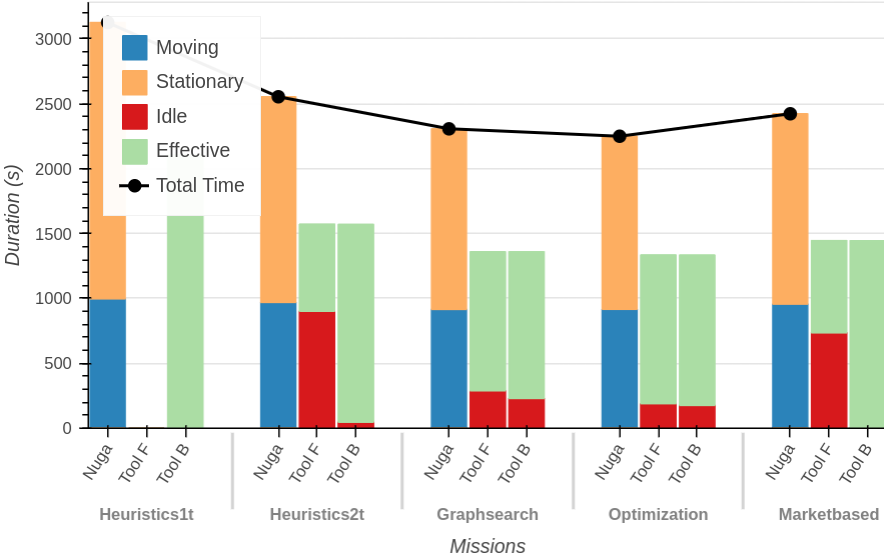
\includegraphics[width=.45\linewidth]{gfx/ch03/50m_medium_density_missions.png}} \\
    \caption{Medium density algorithms comparison}\label{fig:results-medium-density}
\end{figure}

The third simulation corresponds to a weed density of $1.55$ weeds/m$^2$, simulating a high-density scenario, as shown in \autoref{fig:task-visualization-high-density}. Similar to the medium-density scenario (but more pronounced) the graph search and optimization-based approaches show better performance by reducing both mission time and idle time for both tools, achieving balanced tool usage. The market-based algorithm also shows noticeable improvements, achieving better tool productivity and mission time reduction than the baseline, although it still lags behind the other two methods.

\begin{figure}[htb]
    \myfloatalign
    \subfloat[Task Visualization]
    {\label{fig:task-visualization-high-density}
        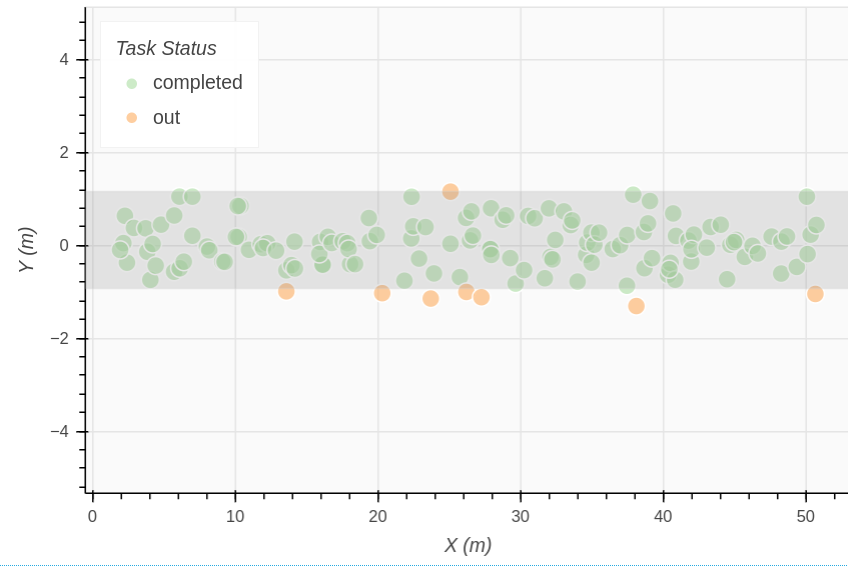
\includegraphics[width=.45\linewidth]{gfx/ch03/50m_high_density_tasks.png}} \quad
    \subfloat[Mission Metrics]
    {\label{fig:mission-metrics-high-density}
        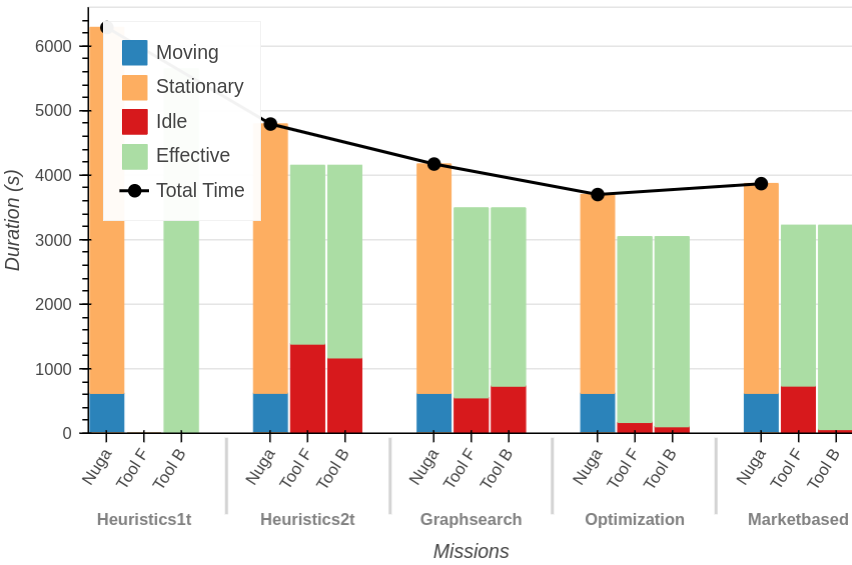
\includegraphics[width=.45\linewidth]{gfx/ch03/50m_high_density_missions.png}} \\
    \caption{High density algorithms comparison}\label{fig:results-high-density}
\end{figure}

The simulation results are summarized in \autoref{tab:low-results}, \autoref{tab:medium-results}, \autoref{tab:high-results} for the low, medium, and high-density simulations, respectively. Each table presents the same information as the previous bar graphs under the '\textit{Raw}' column. Additionally, the '\textit{Improvement}' column shows the relative percentage difference of each algorithm compared to the baseline method for each category. This allows to determine the best algorithm for each weed density scenario.

\begin{table}[H]
    \centering
    \begin{tblr}{
            row{5} = {Silver},
            row{7} = {Silver},
            row{11} = {Silver},
            row{13} = {Silver},
            cell{1}{3} = {c=5}{c},
            cell{1}{8} = {c=5}{c},
            cell{3}{1} = {r=3}{},
            cell{3}{2} = {Silver},
            cell{3}{3} = {Silver},
            cell{3}{4} = {Silver},
            cell{3}{5} = {Silver},
            cell{3}{6} = {Silver},
            cell{3}{7} = {Silver},
            cell{3}{8} = {Silver},
            cell{3}{9} = {Silver},
            cell{3}{10} = {Silver},
            cell{3}{11} = {Silver},
            cell{3}{12} = {Silver},
            cell{6}{1} = {r=3}{},
            cell{6}{8} = {fg=red},
            cell{6}{9} = {fg=JapaneseLaurel},
            cell{6}{10} = {fg=red},
            cell{7}{11} = {fg=JapaneseLaurel},
            % cell{7}{12} = {fg=JapaneseLaurel},
            cell{8}{11} = {fg=red},
            % cell{8}{12} = {fg=red},
            cell{9}{1} = {r=3}{},
            cell{9}{2} = {Silver},
            cell{9}{3} = {Silver},
            cell{9}{4} = {Silver},
            cell{9}{5} = {Silver},
            cell{9}{6} = {Silver},
            cell{9}{7} = {Silver},
            cell{9}{8} = {Silver,fg=red},
            cell{9}{9} = {Silver,fg=JapaneseLaurel},
            cell{9}{10} = {Silver,fg=red},
            cell{9}{11} = {Silver},
            cell{9}{12} = {Silver},
            cell{10}{11} = {fg=JapaneseLaurel},
            % cell{10}{12} = {fg=JapaneseLaurel},
            cell{11}{11} = {fg=red},
            % cell{11}{12} = {fg=red},
            cell{12}{1} = {r=3}{},
            cell{12}{8} = {fg=red},
            cell{12}{9} = {fg=JapaneseLaurel},
            cell{12}{10} = {fg=JapaneseLaurel},
            cell{13}{11} = {fg=JapaneseLaurel},
            % cell{13}{12} = {fg=JapaneseLaurel},
            % cell{14}{12} = {fg=red},
        }
        &    & Raw (min) &       &       &      &      & Improvement (\%) &       &       &        &       \\
        &    & Mov.      & Stat. & Total & Idle & Eff. & Mov.             & Stat. & Total & Idle   & Eff.  \\
        \begin{sideways}Heuristics\end{sideways}   & N  & 15.3      & 16.7  & 32    & -    & -    & -                & -     & -     & -      & -     \\
        & FT & -         & -     & -     & 12.8 & 3.7  & -                & -     & -     & -      & -     \\
        & BT & -         & -     & -     & 0.1  & 16.4 & -                & -     & -     & -      & -     \\
        \begin{sideways}Graph Search\end{sideways} & N  & 16.7      & 16.2  & 32.9  & -    & -    & 9.2              & -3.0  & 2.8   & -      & -     \\
        & FT & -         & -     & -     & 0.1  & 15.7 & -                & -     & -     & -99.2  & 324.3 \\
        & BT & -         & -     & -     & 9.8  & 6.1  & -                & -     & -     & 9700.0 & -62.8 \\
        \begin{sideways}Optimization\end{sideways} & N  & 16.7      & 15.4  & 32.2  & -    & -    & 9.2              & -7.8  & 0.6   & -      & -     \\
        & FT & -         & -     & -     & 0.1  & 14.9 & -                & -     & -     & -99.2  & 302.7 \\
        & BT & -         & -     & -     & 9.8  & 5.3  & -                & -     & -     & 9700.0 & -67.7 \\
        \begin{sideways}Market\end{sideways}       & N  & 15.8      & 14.5  & 30.3  & -    & -    & 3.3              & -13.2 & -5.3  & -      & -     \\
        & FT & -         & -     & -     & 8.3  & 5.9  & -                & -     & -     & -35.2  & 59.5  \\
        & BT & -         & -     & -     & 0.1  & 14.2 & -                & -     & -     & 0.0    & -13.4
    \end{tblr}
    \caption{Low-density Simulation Results}
    \label{tab:low-results}
\end{table}

\paragraph{\autoref{tab:low-results}} Confirms that there is no significant improvement in mission time nor tool productivity when using more sophisticated algorithms in low-density scenarios. We observe that the market-based approach was the only one to achieve a reduction in total mission time, with a $5.3\%$ decrease compared to the baseline method. In contrast, the graph search and optimization methods actually increased the mission time by $2.8\%$ and $0.6\%$, respectively.

Regarding tool productivity, we observe a shift in which tool experiences more idle time: from the front tool in the baseline to the back tool in the cases of graph search and optimization. Despite this shift, both methods reduced the back tool’s idle time from $12.8$ minutes to $9.8$ minutes. The market-based method maintained the front tool as the one with the highest idle time but still achieved a $35.2\%$ reduction.

\begin{table}[H]
    \centering
    \begin{tblr}{
            row{5} = {Silver},
            row{7} = {Silver},
            row{11} = {Silver},
            row{13} = {Silver},
            cell{1}{3} = {c=5}{c},
            cell{1}{8} = {c=5}{c},
            cell{3}{1} = {r=3}{},
            cell{3}{2} = {Silver},
            cell{3}{3} = {Silver},
            cell{3}{4} = {Silver},
            cell{3}{5} = {Silver},
            cell{3}{6} = {Silver},
            cell{3}{7} = {Silver},
            cell{3}{8} = {Silver},
            cell{3}{9} = {Silver},
            cell{3}{10} = {Silver},
            cell{3}{11} = {Silver},
            cell{3}{12} = {Silver},
            cell{6}{1} = {r=3}{},
            cell{6}{8} = {fg=JapaneseLaurel},
            cell{6}{9} = {fg=JapaneseLaurel},
            cell{6}{10} = {fg=JapaneseLaurel},
            cell{7}{11} = {fg=JapaneseLaurel},
            % cell{7}{12} = {fg=JapaneseLaurel},
            cell{8}{11} = {fg=red},
            % cell{8}{12} = {fg=red},
            cell{9}{1} = {r=3}{},
            cell{9}{2} = {Silver},
            cell{9}{3} = {Silver},
            cell{9}{4} = {Silver},
            cell{9}{5} = {Silver},
            cell{9}{6} = {Silver},
            cell{9}{7} = {Silver},
            cell{9}{8} = {Silver,fg=JapaneseLaurel},
            cell{9}{9} = {Silver,fg=JapaneseLaurel},
            cell{9}{10} = {Silver,fg=JapaneseLaurel},
            cell{9}{11} = {Silver},
            cell{9}{12} = {Silver},
            cell{10}{11} = {fg=JapaneseLaurel},
            % cell{10}{12} = {fg=JapaneseLaurel},
            cell{11}{11} = {fg=red},
            % cell{11}{12} = {fg=red},
            cell{12}{1} = {r=3}{},
            cell{12}{8} = {fg=JapaneseLaurel},
            cell{12}{9} = {fg=JapaneseLaurel},
            cell{12}{10} = {fg=JapaneseLaurel},
            cell{13}{11} = {fg=JapaneseLaurel},
            % cell{13}{12} = {fg=JapaneseLaurel},
            cell{14}{11} = {fg=JapaneseLaurel},
            % cell{14}{12} = {fg=red},
        }
        &    & Raw (min) &       &       &      &      & Improvement (\%) &       &       &        &       \\
        &    & Mov.      & Stat. & Total & Idle & Eff. & Mov.             & Stat. & Total & Idle   & Eff.  \\
        \begin{sideways}Heuristics\end{sideways}   & N  & 16.1      & 26.4  & 42.5  & -    & -    & -                & -     & -     & -      & -     \\
        & FT & -         & -     & -     & 15   & 11.1 & -                & -     & -     & -      & -     \\
        & BT & -         & -     & -     & 0.7  & 25.3 & -                & -     & -     & -      & -     \\
        \begin{sideways}Graph Search\end{sideways} & N  & 15.2      & 23.1  & 38.4  & -    & -    & -5.6             & -12.5 & -9.6  & -      & -     \\
        & FT & -         & -     & -     & 4.8  & 17.8 & -                & -     & -     & -68.0  & 60.4  \\
        & BT & -         & -     & -     & 3.8  & 18.8 & -                & -     & -     & 442.9  & -25.7 \\
        \begin{sideways}Optimization\end{sideways} & N  & 16        & 24.5  & 40.6  & -    & -    & -0.6             & -7.2  & -4.5  & -      & -     \\
        & FT & -         & -     & -     & 1.7  & 22.4 & -                & -     & -     & -88.7  & 101.8 \\
        & BT & -         & -     & -     & 9.8  & 14.2 & -                & -     & -     & 1300.0 & -43.9 \\
        \begin{sideways}Market\end{sideways}       & N  & 15.9      & 24.4  & 40.3  & -    & -    & -1.2             & -7.6  & -5.2  & -      & -     \\
        & FT & -         & -     & -     & 12.2 & 11.8 & -                & -     & -     & -18.7  & 6.3   \\
        & BT & -         & -     & -     & 0    & 24   & -                & -     & -     & -100.0 & -5.1
    \end{tblr}
    \caption{Medium-density Simulation Results}
    \label{tab:medium-results}
\end{table}

\begin{table}[H]
    \centering
    \begin{tblr}{
            row{4} = {c},
            row{5} = {Silver,c},
            row{7} = {Silver,c},
            row{8} = {c},
            row{10} = {c},
            row{11} = {Silver,c},
            row{13} = {Silver,c},
            row{14} = {c},
            cell{1}{3} = {c=5}{c},
            cell{1}{8} = {c=5}{c},
            cell{3}{1} = {r=3}{},
            cell{3}{2} = {Silver,c},
            cell{3}{3} = {Silver,c},
            cell{3}{4} = {Silver,c},
            cell{3}{5} = {Silver,c},
            cell{3}{6} = {Silver,c},
            cell{3}{7} = {Silver,c},
            cell{3}{8} = {Silver,c},
            cell{3}{9} = {Silver,c},
            cell{3}{10} = {Silver,c},
            cell{3}{11} = {Silver,c},
            cell{3}{12} = {Silver,c},
            cell{6}{1} = {r=3}{},
            cell{6}{2} = {c},
            cell{6}{3} = {c},
            cell{6}{4} = {c},
            cell{6}{5} = {c},
            cell{6}{6} = {c},
            cell{6}{7} = {c},
            cell{6}{8} = {c},
            cell{6}{9} = {c,fg=JapaneseLaurel},
            cell{6}{10} = {c,fg=JapaneseLaurel},
            cell{6}{11} = {c},
            cell{6}{12} = {c},
            cell{7}{11} = {fg=JapaneseLaurel},
            % cell{7}{12} = {fg=JapaneseLaurel},
            cell{8}{11} = {fg=JapaneseLaurel},
            % cell{8}{12} = {fg=red},
            cell{9}{1} = {r=3}{},
            cell{9}{2} = {Silver,c},
            cell{9}{3} = {Silver,c},
            cell{9}{4} = {Silver,c},
            cell{9}{5} = {Silver,c},
            cell{9}{6} = {Silver,c},
            cell{9}{7} = {Silver,c},
            cell{9}{8} = {Silver,c},
            cell{9}{9} = {Silver,c,fg=JapaneseLaurel},
            cell{9}{10} = {Silver,c,fg=JapaneseLaurel},
            cell{9}{11} = {Silver,c},
            cell{9}{12} = {Silver,c},
            cell{10}{11} = {fg=JapaneseLaurel},
            % cell{10}{12} = {fg=JapaneseLaurel},
            cell{11}{11} = {fg=JapaneseLaurel},
            % cell{11}{12} = {fg=red},
            cell{12}{1} = {r=3}{},
            cell{12}{2} = {c},
            cell{12}{3} = {c},
            cell{12}{4} = {c},
            cell{12}{5} = {c},
            cell{12}{6} = {c},
            cell{12}{7} = {c},
            cell{12}{8} = {c},
            cell{12}{9} = {c,fg=JapaneseLaurel},
            cell{12}{10} = {c,fg=JapaneseLaurel},
            cell{12}{11} = {c},
            cell{12}{12} = {c},
            cell{13}{11} = {fg=JapaneseLaurel},
            % cell{13}{12} = {fg=red},
            cell{14}{11} = {fg=JapaneseLaurel},
            % cell{14}{12} = {fg=JapaneseLaurel},
        }
        &    & Raw (min) &       &       &      &      & Improvement (\%) &       &       &       &       \\
        &    & Mov.      & Stat. & Total & Idle & Eff. & Mov.             & Stat. & Total & Idle  & Eff.  \\
        \begin{sideways}Heuristics\end{sideways}   & N  & 10.3      & 69.4  & 79.8  & -    & -    & -                & -     & -     & -     & -     \\
        & FT & -         & -     & -     & 23   & 46   & -                & -     & -     & -     & -     \\
        & BT & -         & -     & -     & 19.5 & 49.6 & -                & -     & -     & -     & -     \\
        \begin{sideways}Graph Search\end{sideways} & N  & 10.3      & 59.1  & 69.4  & -    & -    & 0.0              & -14.8 & -13.0 & -     & -     \\
        & FT & -         & -     & -     & 9.1  & 48.9 & -                & -     & -     & -60.4 & 6.3   \\
        & BT & -         & -     & -     & 12.1 & 45.9 & -                & -     & -     & -37.9 & -7.5  \\
        \begin{sideways}Optimization\end{sideways} & N  & 10.3      & 51.2  & 61.6  & -    & -    & 0.0              & -26.2 & -22.8 & -     & -     \\
        & FT & -         & -     & -     & 2.8  & 47.8 & -                & -     & -     & -87.8 & 3.9   \\
        & BT & -         & -     & -     & 1.7  & 48.9 & -                & -     & -     & -91.3 & -1.4  \\
        \begin{sideways}Market\end{sideways}       & N  & 10.3      & 54    & 64.4  & -    & -    & 0.0              & -22.2 & -19.3 & -     & -     \\
        & FT & -         & -     & -     & 12.2 & 41.4 & -                & -     & -     & -47.0 & -10.0 \\
        & BT & -         & -     & -     & 1    & 52.6 & -                & -     & -     & -94.9 & 6.0
    \end{tblr}
    \caption{High-density Simulation Results}
    \label{tab:high-results}
\end{table}

\paragraph{\autoref{tab:medium-results}} Highlights the improvements achieved in medium-density scenarios by the implemented algorithms over the heuristic approach. The graph search, optimization, and market-based methods reduced mission time by $9.6\%$, $4.5\%$, and $5.2\%$, respectively. Additionally, they achieved more balanced tool usage and reductions in idle time up to $88.7\%$ for the front tool. The observed increment in back tool idle time is attributed to the heuristic method’s unbalanced tool usage, which resulted in a very low idle time for only one tool, which is not desired.

\paragraph{\autoref{tab:high-results}} Demonstrates the effectiveness of the proposed algorithms in high-density scenarios. The graph search, optimization, and market-based methods achieved mission time reductions of $13.0\%$, $22.8\%$, and $19.3\%$, respectively. In terms of tool usage, all three methods achieved a balanced tool usage, with reductions in idle time of up to $87.8\%$ for the front tool and up to $94.9\%$ for the back tool.

\subsection{Computation Time}\label{sec:computation-time}
The heuristic and market-based algorithms are considered shortsighted in nature due to the way they compute the next best stop without considering all tasks available up to that point. This characteristic makes their computation time negligible, regardless of the number of tasks currently available. In contrast, graph search and optimization-based algorithms take all available information into account when computing a solution, resulting in a larger solution space and, consequently, greater computational time required.

Our graph search solution performs well in terms of computation time, for a low to medium density of weeds. However, as the number of weeds increases, the graph size grows exponentially, leading to longer computation times. \autoref{fig:graphsearch-performance} showcases the graph size and computation time for different number of weeds (see plot in red). The graph size is defined as the number of nodes in the graph, while the computation time is the time required to build and find the optimal path in the graph.

\begin{figure}[htb]
    \myfloatalign
    \subfloat[Graph size vs. number of weeds]
    {\label{fig:graphsearch-graph-size}%
        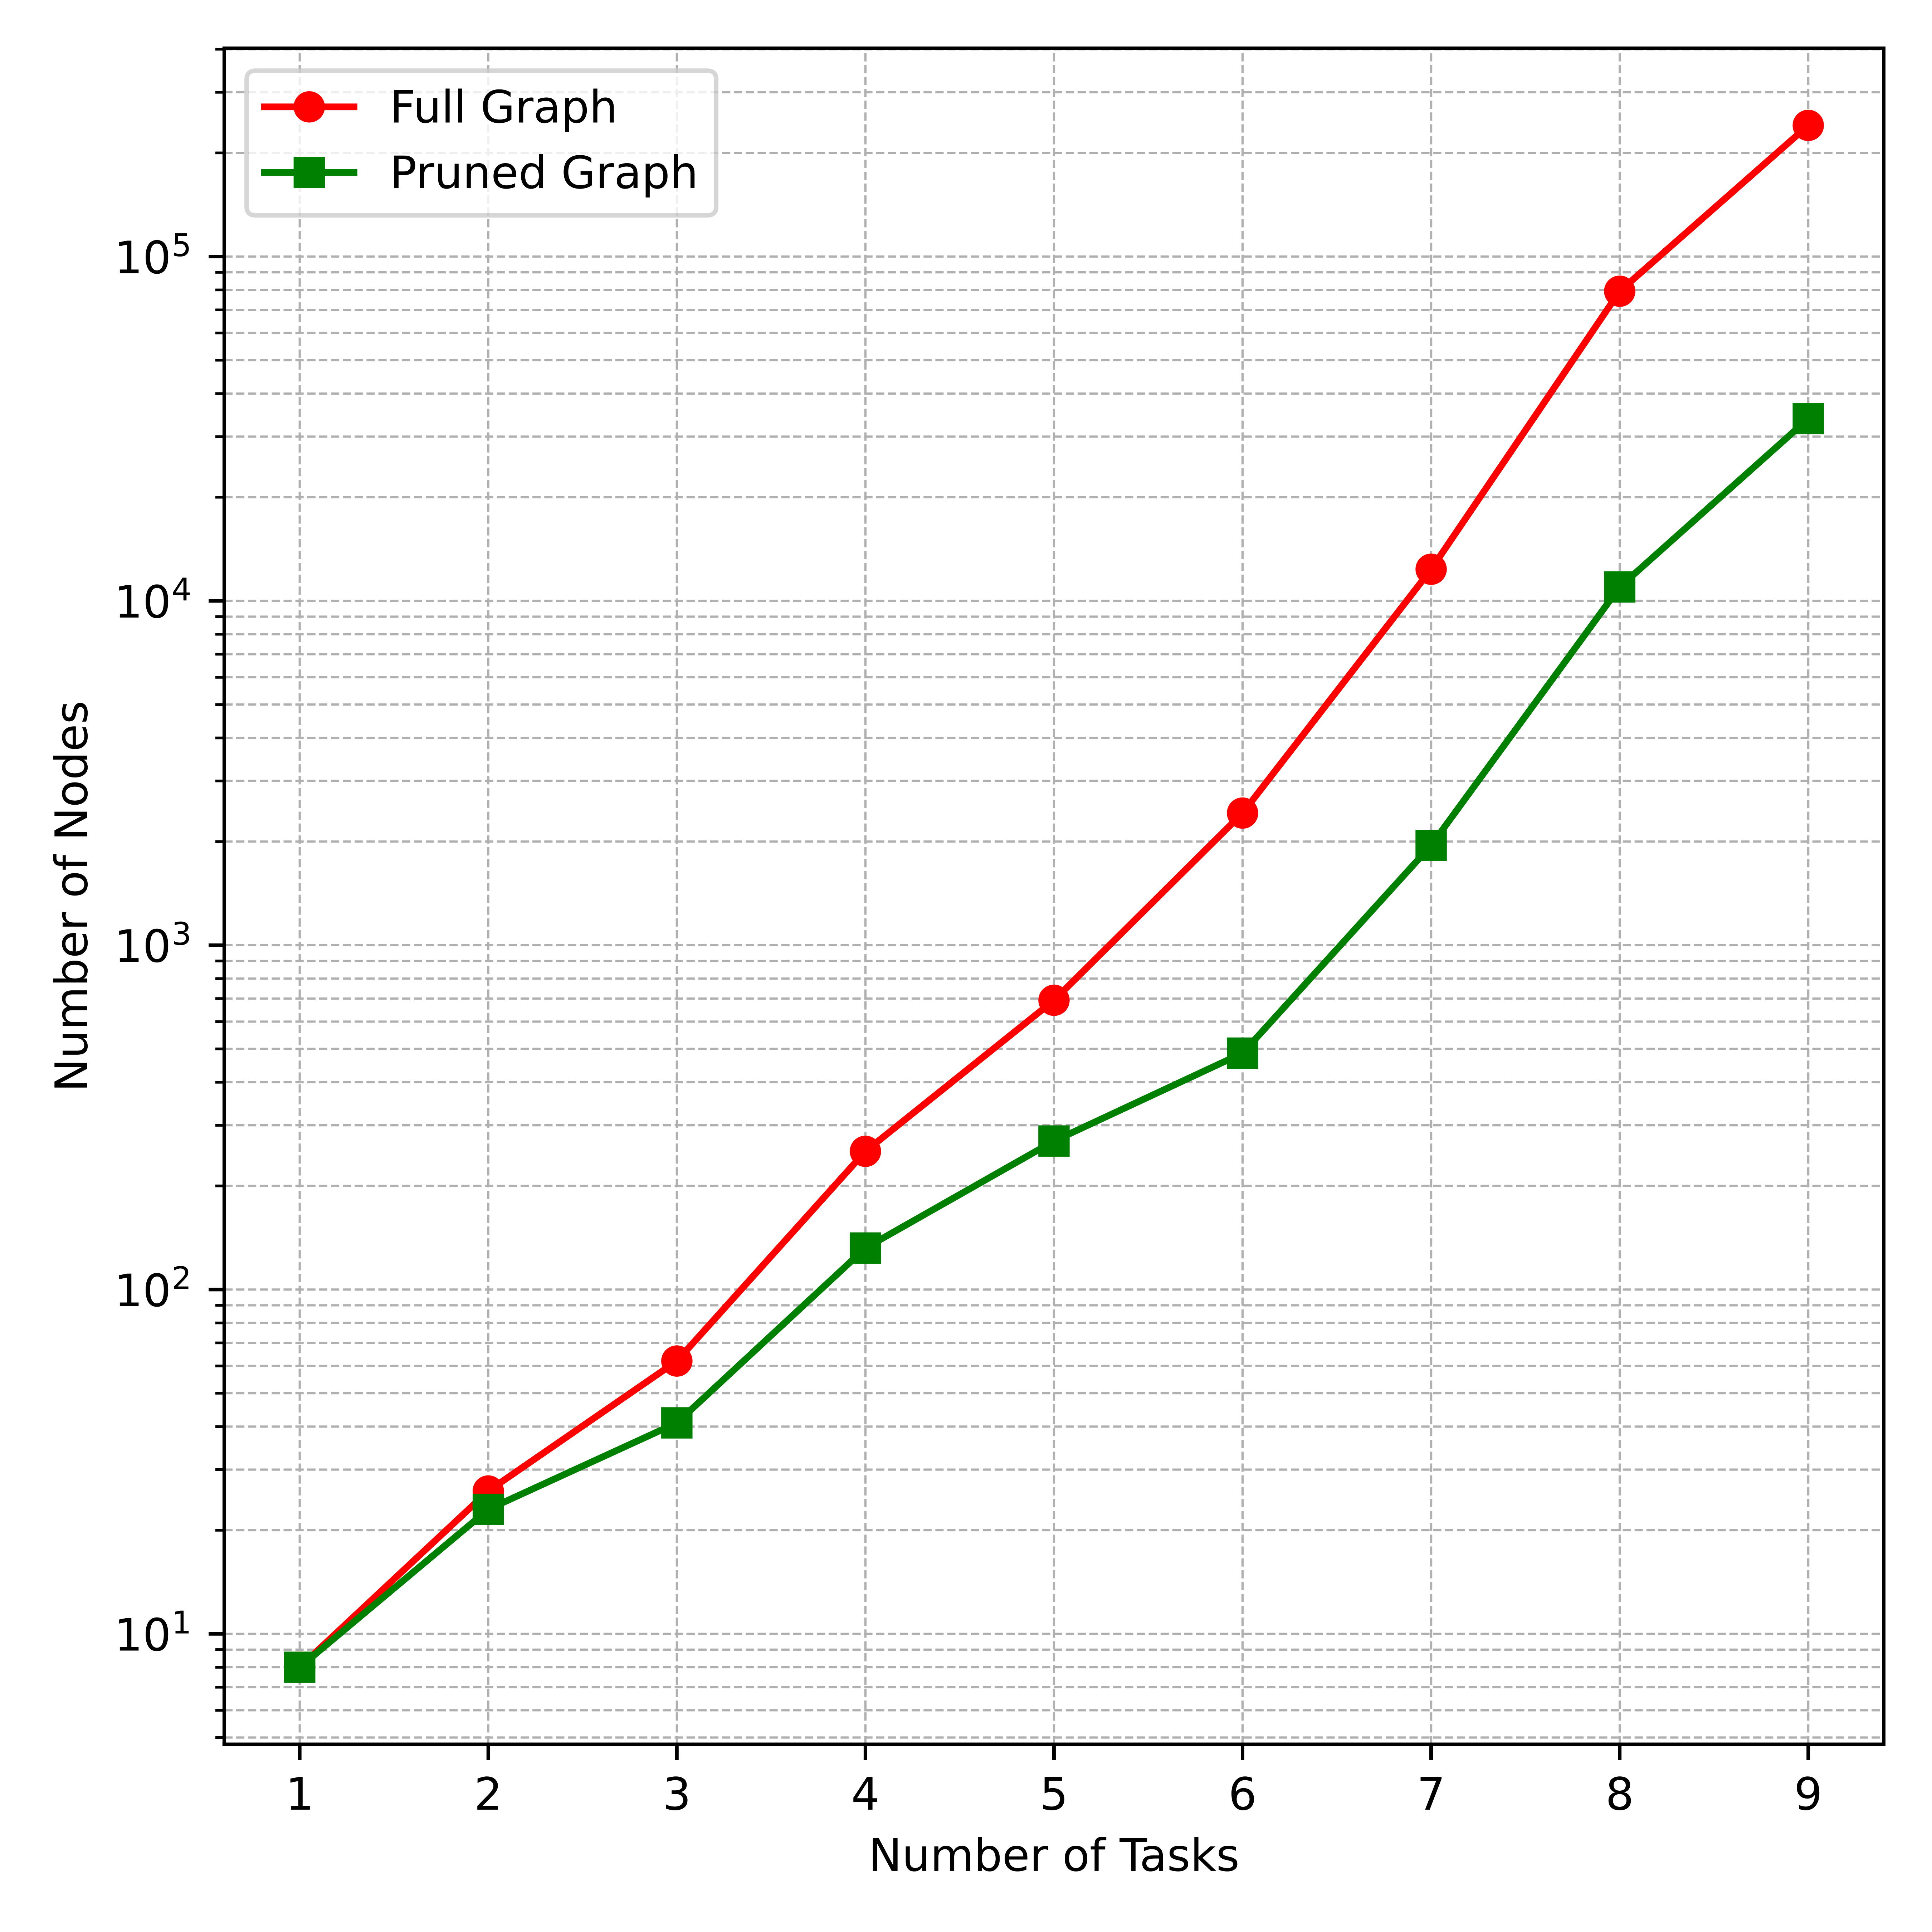
\includegraphics[width=.45\linewidth]{gfx/ch03/gs_graph_size_plot.png}} \quad
    \subfloat[Processing time vs. number of weeds]
    {\label{fig:graphsearch-processing-time}%
        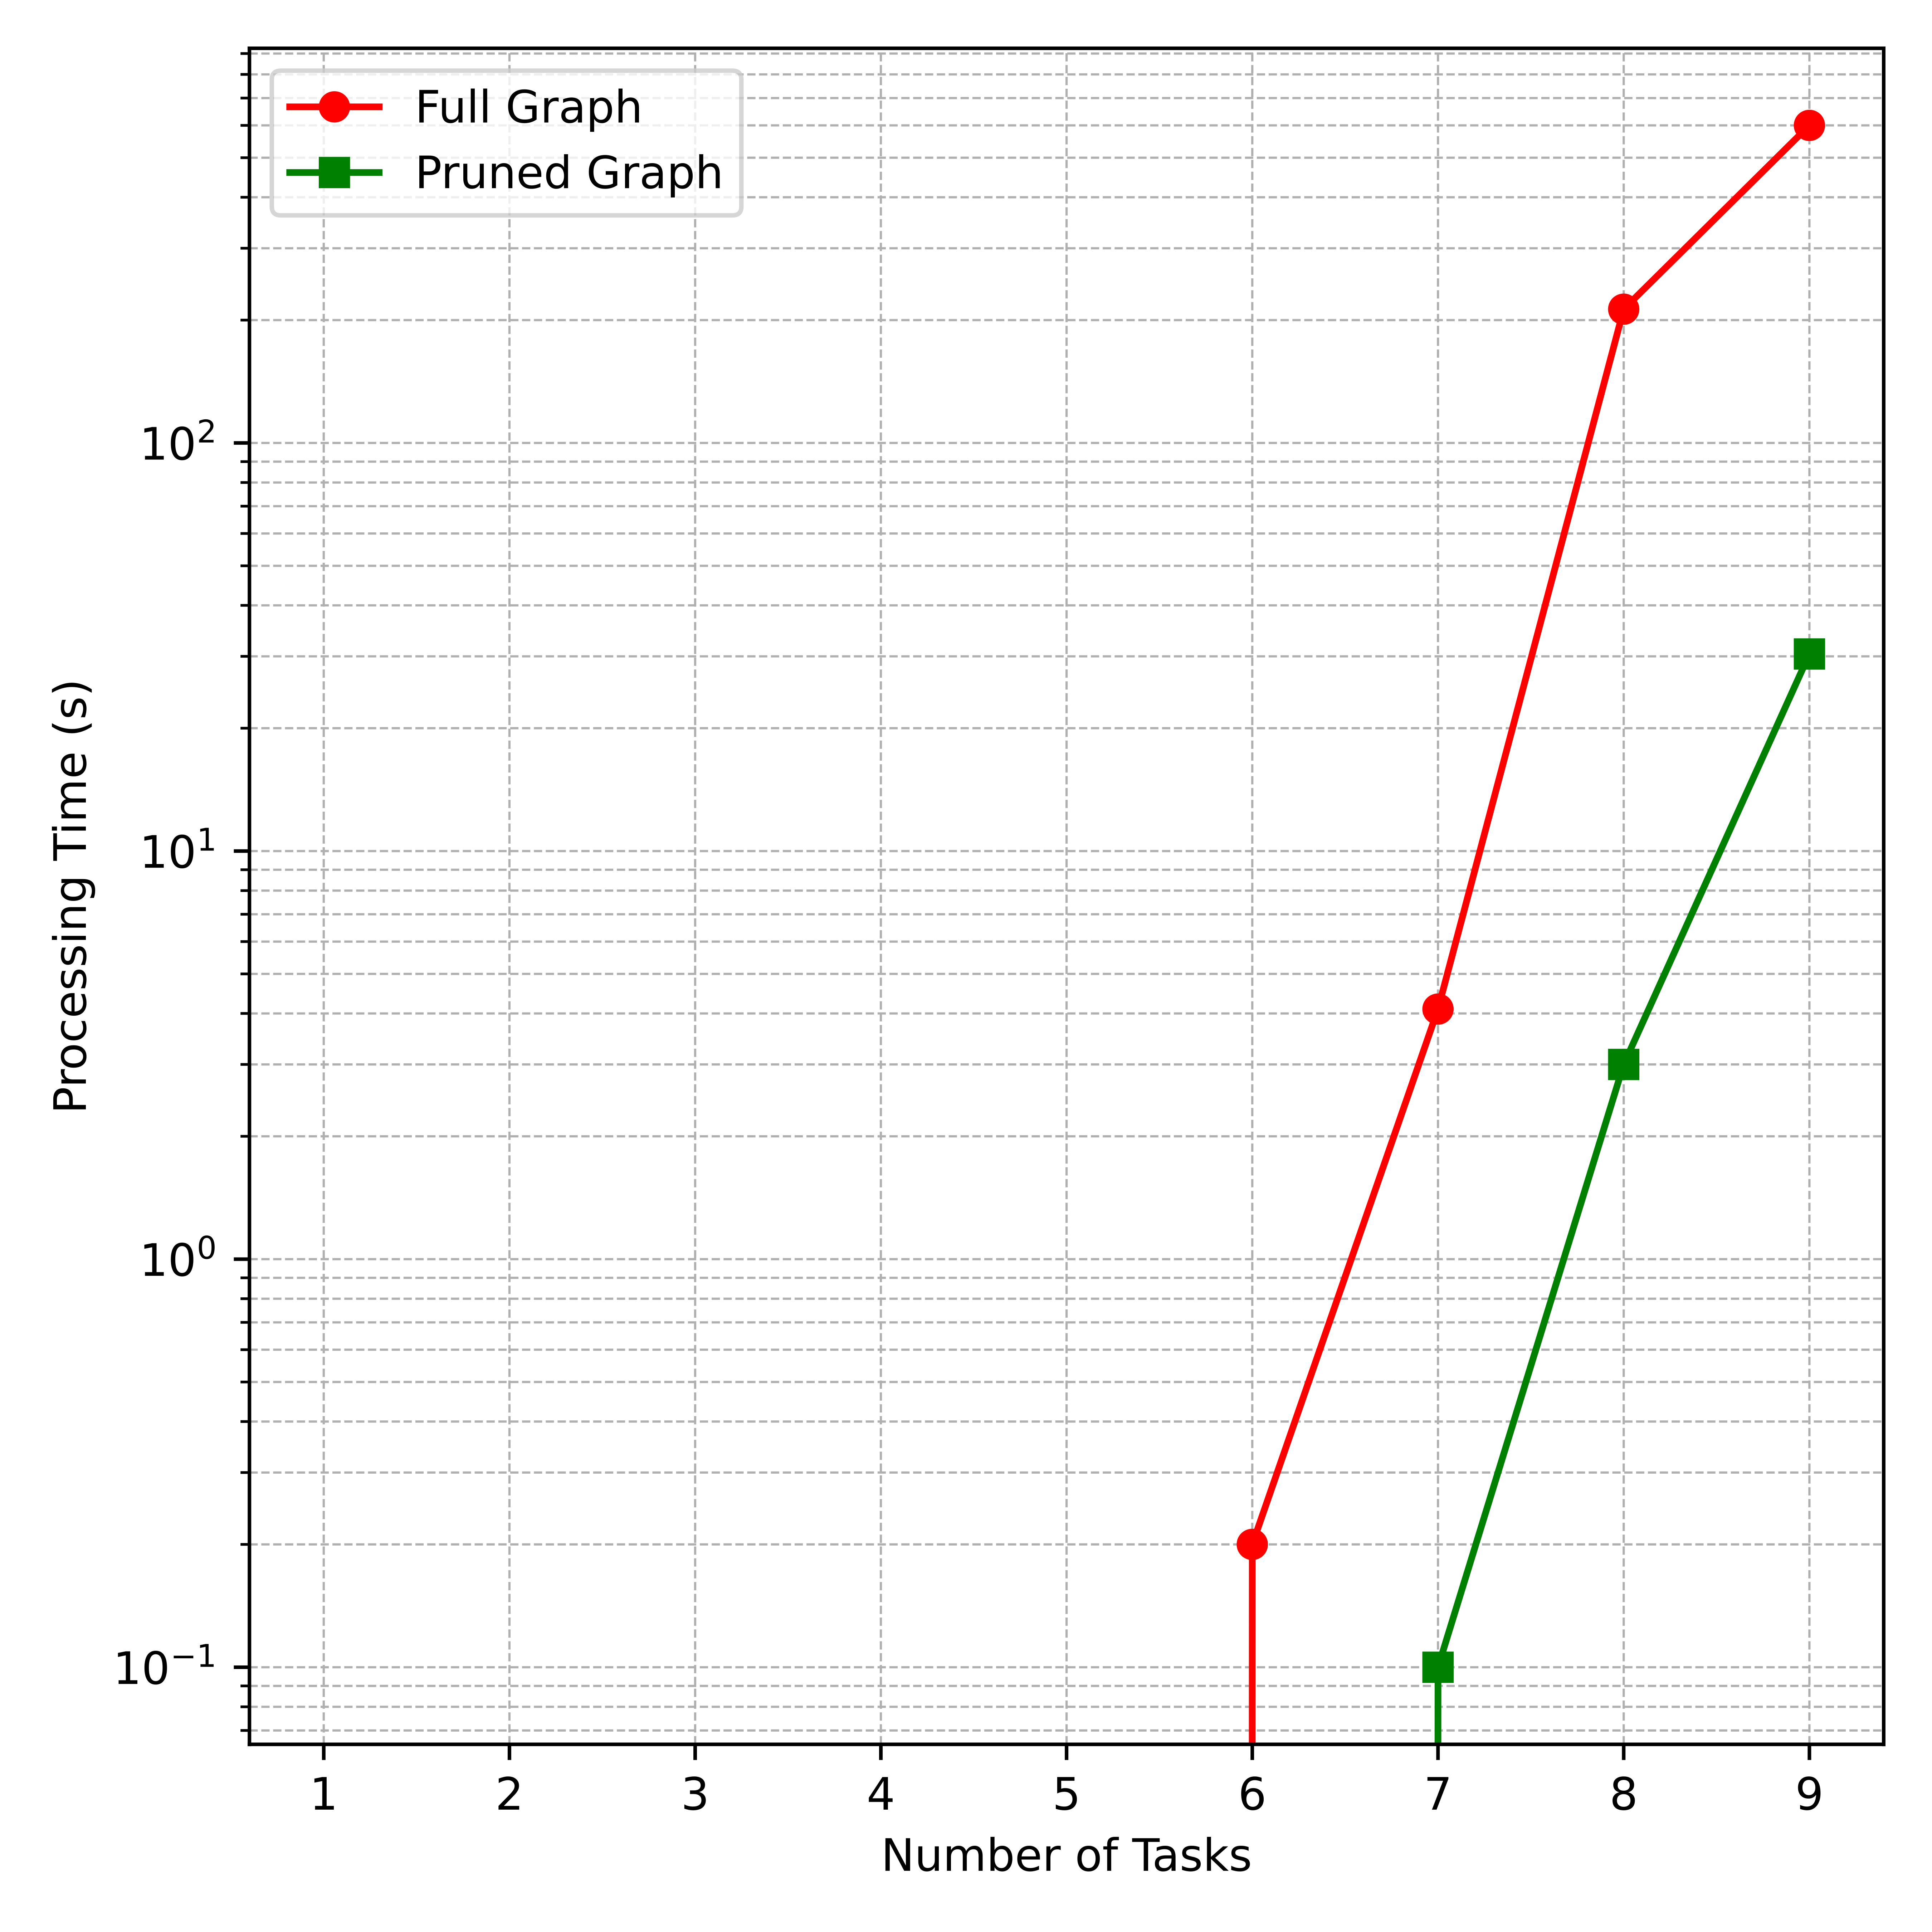
\includegraphics[width=.45\linewidth]{gfx/ch03/gs_proce_time_plot.png}} \\
    \caption{Graph Search algorithm performance}\label{fig:graphsearch-performance}
\end{figure}

We were able to optimize and reduce the graph size by applying a pruning technique that stops the growth of certain branches when they are not promising. This is achieved by introducing the concept of \textit{expired tasks}, these are tasks that haven't been removed and can no longer be removed in future stops because the corresponding weeds have been left behind, outside the tool's workspaces. This pruning is implemented in the \texttt{get\_children\_nodes} method, where each task is checked for expiration before being added to the graph. As a result, the number of nodes is significantly reduced, improving computation time (observe green plot in \autoref{fig:graphsearch-performance}).

A similar processing time analysis was conducted for the optimization-based algorithm. Unlike the graph search approach, its computation time scales well with the number of tasks and does not exhibit the same performance issues. This comparison is illustrated in \autoref{fig:mip-vs-gs-processing-time}. Note that graph search is only a feasible solution for up to 10 tasks, beyond this point, the processing time becomes too high for practical use in online applications. In contrast, the optimization-based approach remains feasible for handling up to 300 tasks at a time.

\begin{figure}[hbt]
    \centering
    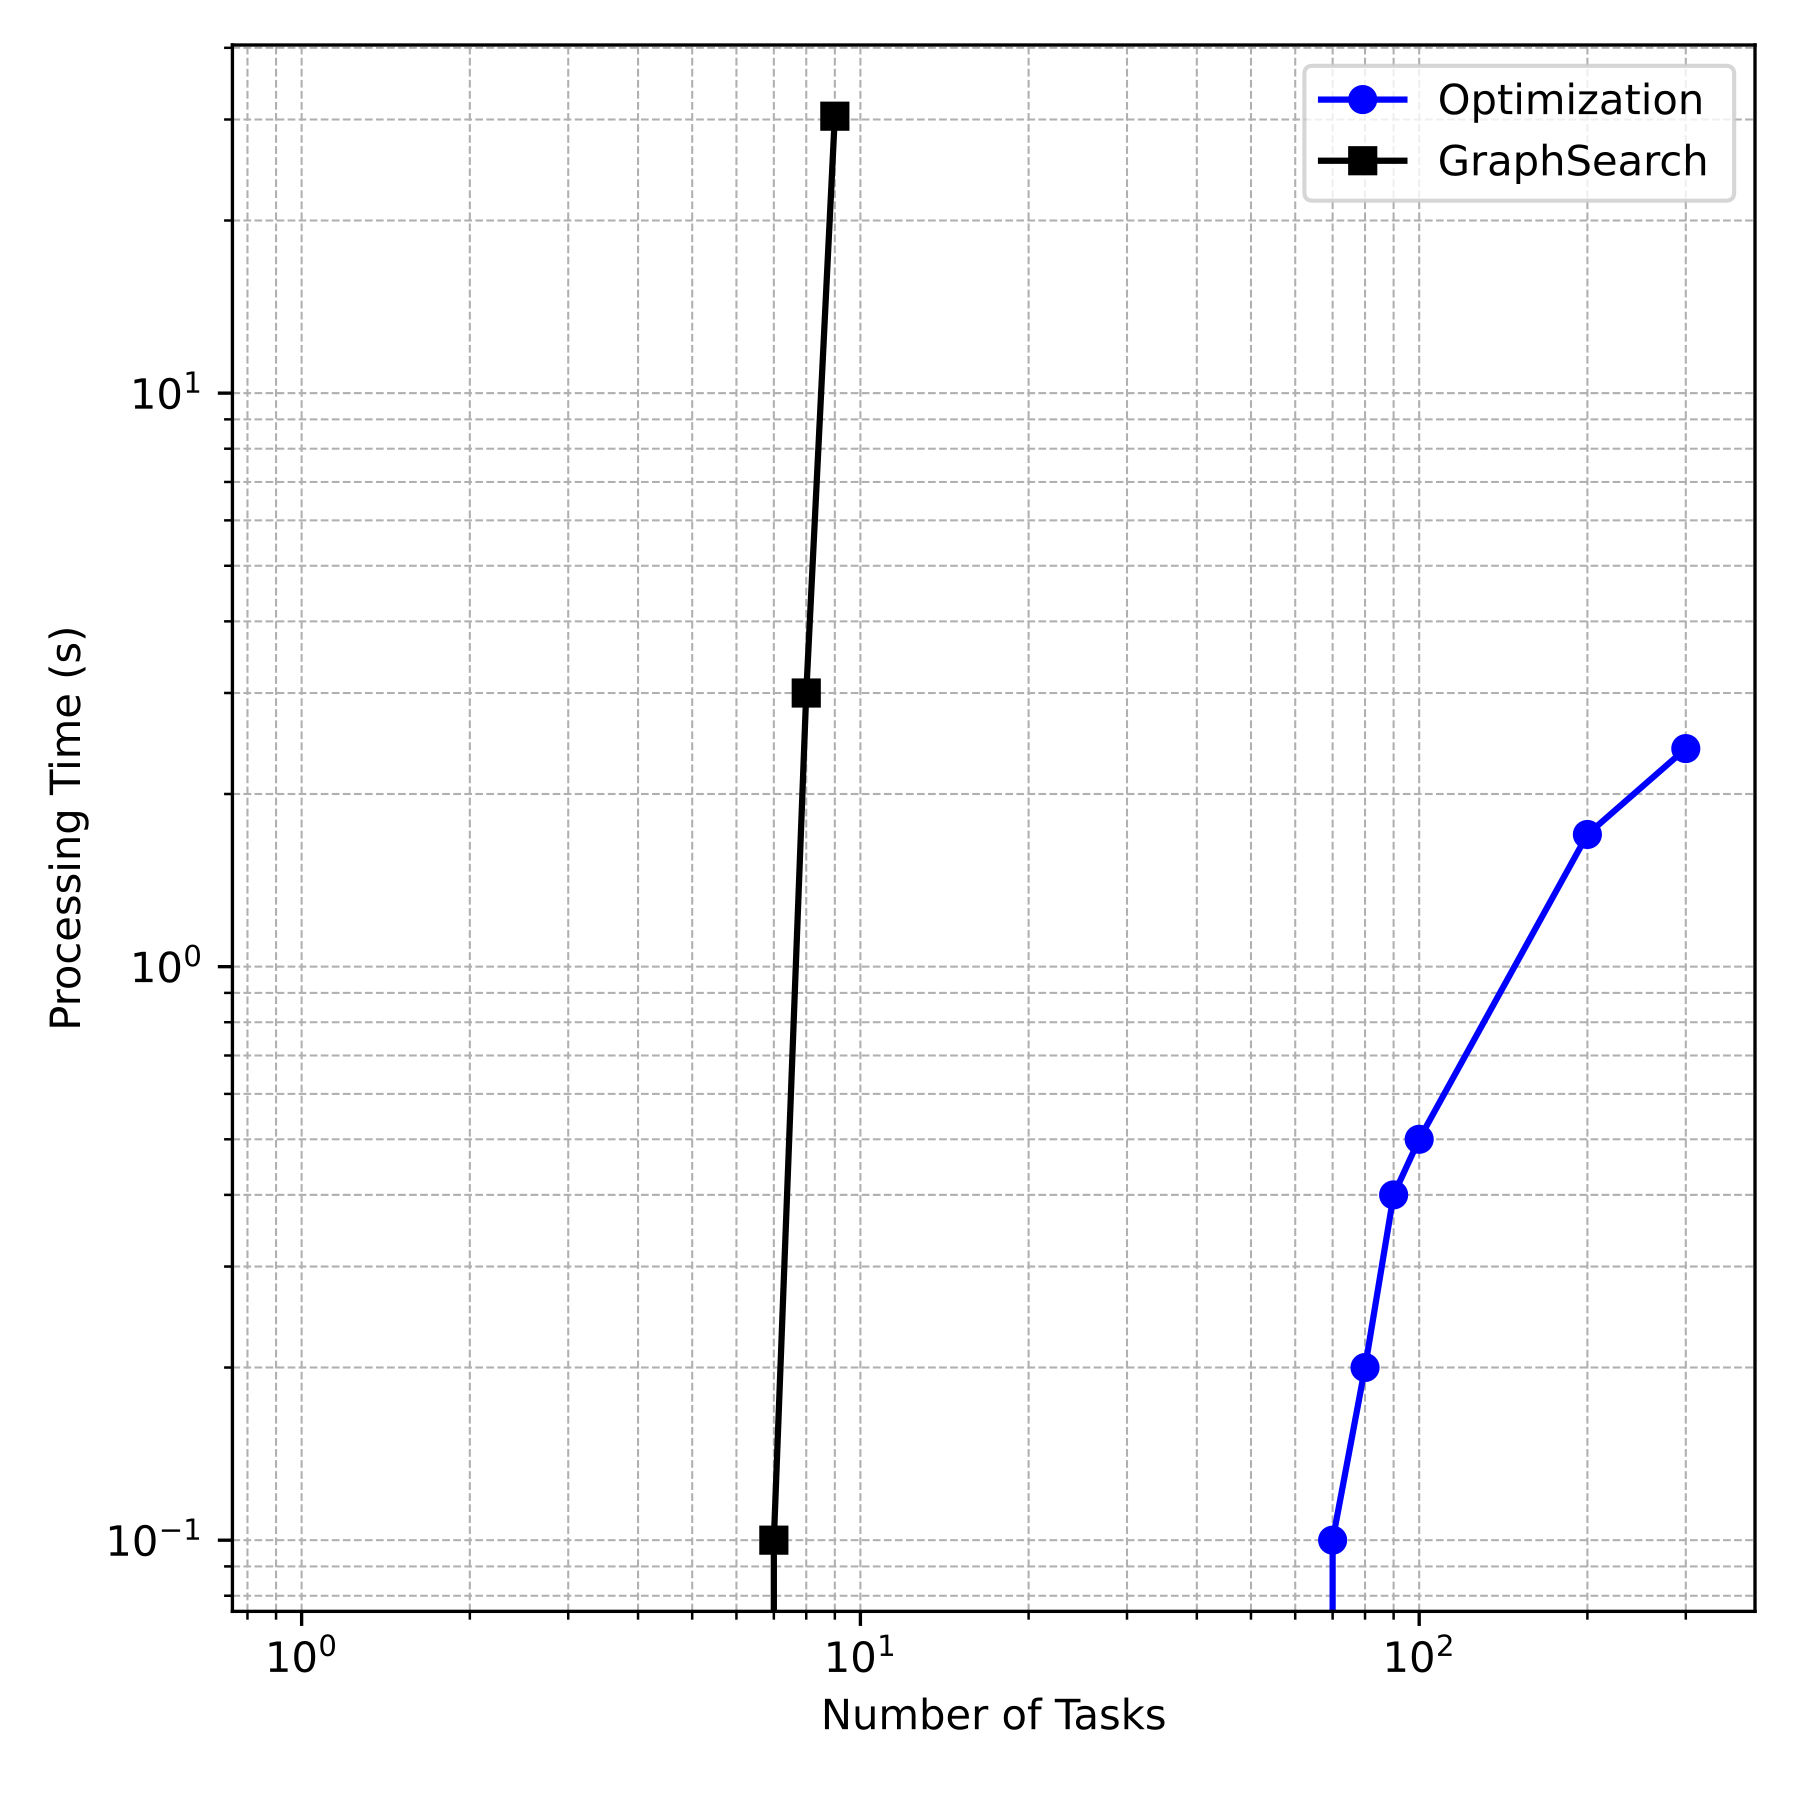
\includegraphics[width=0.5\linewidth]{gfx/ch03/mip_vs_gs_procc_time_plot.png}
    \caption{Graph Search vs. Optimization}
    \label{fig:mip-vs-gs-processing-time}
\end{figure}

\subsection{Future Work}
Observing improvements in mission duration and reduced idle time by adding an additional tool to the system and selecting the appropriate \ac{TA} algorithm raises important questions such as: \textit{To what extent does increasing the number of \ac{IT} improve mission productivity?} \textit{Is the cost-productivity trade-off justified when using more than two onboard tools?}. The simulation developed in this thesis lays the foundation for answering such questions. By varying the number of \ac{IT} and collecting comparative performance data, these analyses could be carried out if Paltech chooses to pursue them.

On another note, the dynamic nature of the task allocation problem means that information becomes available progressively as the mission takes place. Therefore, it is important to recognize that the solutions obtained are \textbf{locally optimal} based on currently available information. If the algorithm had access to all task information from the start, the likelihood of finding \textbf{globally optimal solutions} would be significantly higher. Questions such as \textit{how much better those solutions would be}, and \textit{what trade-offs they would involve}, remain open and are worth exploring. However, this scenario is hypothetical due to current hardware constraints, specifically, the limited field of view of the camera. The possibility of detecting tasks farther ahead, either through hardware changes or different sensing approaches, could provide the algorithm with more foresight, leading to better solutions. Investigating such enhancements is proposed as future work.

%*****************************************
%*****************************************
%*****************************************
%*****************************************
%*****************************************
